\documentclass[office, 10pt, openany]{book}
\usepackage{trackchanges}
% idioma
\usepackage[utf8]{inputenc}
\usepackage[USenglish,british,american,australian,english]{babel}
%tablas
\usepackage{booktabs}
\usepackage{tabularx}
%rotar tablas
\usepackage{rotating}
%Manejo de referencias
%\usepackage[style=mla]{biblatex}
%color tablas
\usepackage{colortbl}
%espaciado
\usepackage{setspace}
\onehalfspacing
\setlength{\parindent}{0pt}
\setlength{\parskip}{2.0ex plus0.5ex minus0.2ex}
% Default fixed font does not support bold face
\DeclareFixedFont{\ttb}{T1}{txtt}{bx}{n}{8} % for bold
\DeclareFixedFont{\ttm}{T1}{txtt}{m}{n}{8}  % for normal

% Custom colors
\usepackage{color}
\definecolor{deepblue}{rgb}{0,0,0.5}
\definecolor{deepred}{rgb}{0.6,0,0}
\definecolor{deepgreen}{rgb}{0,0.5,0}

\usepackage{listings}



%margenes segun n. icontec
\usepackage{vmargin}
\setmarginsrb           { 3.0cm}  % left margin
                        { 4.0cm}  % top margcm
                        { 3.0cm}  % right margcm
                        { 3.0cm}  % bottom margcm
                        {  10pt}  % head height
                        {0.25cm}  % head sep
                        {   9pt}  % foot height
                        { 0.3cm}  % foot sep


% insercion url's notas de pie.
\usepackage{url}
%\usepackage{hyperref}
% Paquetes de la AMS:
\usepackage{amsmath, amsthm, amsfonts, amssymb}

%---- New commands

\newcommand\portada{
\begin{titlepage}
		\begin{center}
			{\large \bf  A Software Platform For The Simulation Of Light Propagation In Photonic Crystal Structures With Defects}
			\vfill
			{\large\bf Santiago Echeverri Chac\'on
			\\\emph{sechev14@eafit.edu.co}\par}
%			{\large\bf Advisor: Nicol\'as Guar\'in Zapata
%			\\\emph{nicoguarin@gmail.com}}
			\vfill
								\vfill
			{\large\bf Departamento de Ciencias B\'asicas \par}
			{\large\bf Escuela de Ciencias y Humanidades \par}
			{\large\bf Universidad EAFIT \par}
			{\large\bf Medell\'in, Colombia\par}
			{\large\bf May 2013 \par}
		\end{center}
\end{titlepage}
}

\newcommand\contraportada{
	\begin{titlepage}
		\begin{center}
			{\large \bf A Software Platform For The Simulation Of Light Propagation In Photonic Crystal Structures With Defects} 
			\vfill
% 			{\large\bf PRESENTADO POR \par}
			{\large\bf Santiago Echeverri Chac\'on
			\\\emph{sechev14@eafit.edu.co}\par}
			{\large\bf Advisor: Nicol\'as Guar\'in Zapata
			\\\emph{nicoguarin@gmail.com}}
			\vfill
			{\large\bf Thesis document presented as a partial prerequisite for the title of Bachelor in Engineering Physics \par}
			\vfill
			\vfill
			{\large\bf Departamento de Ciencias B\'asicas \par}
			{\large\bf Escuela de Ciencias y Humanidades \par}
			{\large\bf Universidad EAFIT \par}
			{\large\bf Medell\'in, Colombia\par}
			{\large\bf May 2013 \par}
		\end{center}
\end{titlepage}
}


% Python style for highlighting
\newcommand\pythonstyle{\lstset{
language=Python,
basicstyle=\ttm,
otherkeywords={self},             % Add keywords here
keywordstyle=\ttb\color{deepblue},
emph={MyClass,__init__},          % Custom highlighting
emphstyle=\ttb\color{deepred},    % Custom highlighting style
stringstyle=\color{deepgreen},
frame=tb,                         % Any extra options here
showstringspaces=false            % 
}}
% Python environment
\lstnewenvironment{python}[1][]
{
\pythonstyle
\lstset{#1}
}
{}

%---- End of New commands 

%--------------------------------------------------------------------------
% \title{\LARGE \bf Plantilla para un artculo \LaTeX }
% % \vfill
% \author{El autor va aqui
%   \small Dept. Plantillas y Editores\\
%   \small E12345\\
%   \small Espaa
% }
%Para incluir detalles cucas del pdf
\usepackage[pdftex, pdftitle={A Software Platform For The Simulation Of Light Propagation In Photonic Crystal Structures With Defects}, pdfauthor={Santiago Echeverri},
pdfsubject={Photonic Crystals numerical modeling}, pdfkeywords={Numerical methods, computational photonics, photonic crystal defects}, pdfpagemode=UseOutlines,bookmarks,bookmarksopen,pdfstartview=FitH,colorlinks,linkcolor=blue,
urlcolor=blue, cite color=blue]{hyperref} %
\usepackage[hyperpageref]{backref} 
\begin{document}
\portada
\cleardoublepage
\contraportada

\pdfbookmark[0]{Table of contents}{}
\tableofcontents
\listoffigures
\clearpage

\chapter{Introduction}

\note[NGZ]{La introduccion es lo que motiva al lector a leer el documento. Debe responder las preguntas: Por qu\'e es relevante esto?, Por qu\'e es relevante que yo (como ingeniero f\'isico) lo haya abordado?, Qu\'e componentes de ingenier\'ia y de f\'isica se han tocado en el trabajo?}
Preface:

Definition of the problem will be treated in chapter \ref{ch:Problem}, followed by a brief state of the art recollection where some background in the topics of photonic crystals and computational methods for physics will be mentioned. Then, fundamental concepts behind light propagation in periodic materials (chapter \ref{ch:Electromagnetic waves in periodic media})  and the model used for the finite element procedure used are presented.
\chapter{Problem}
\label{ch:Problem}

\section{Problem statement}

This project aims to develop a simulation software package that permits analysis of electromagnetic (EM) wave propagation, in the context of Photonic Crystal (PC) defects modelling and design.

%Problem statement will herein be addressed as the goal of the project.
% Being so it is an abstraction of what has to be accomplished.
% Objectives, which are to be addressed next reffer to the specifics of the problem statment
% It is very likely that the problem statement and a general objective be confused, actiually I do. Maybe they are the same. I address this confusion here making the general objective a bit more implementation-oriented.
\section{Objectives }

\subsection{General objectives}
\begin{itemize}
\item Build a software platform capable of simulating   electromagnetic field propagation in perfect PC and also in PC with defects such as cavities and inclusions.
\item The platform architecture must be structured in a way that facilitates future upgrading, possible optimization schemes, and integration with other kinds of simulations like confinement of electrons in potential wells and crystals. 
\end{itemize}

% Objectives must be S.M.A.R.T:
% Specific, Measurable, Achievable, Relevant and Time-bound.%


\subsubsection{Specific objectives}
\begin{enumerate}
\item  Apprehend the theory behind EM fields and its applications in photonics. Particularly: 
\begin{enumerate}
	 \item general overview of computational methods in electromagnetism and deeper understanding of methods that fit the problem statement.
	 \item Photonic crystals and the mathematical tools for modeling periodicity, as well as 
	 \item technological applications of defects in photonic crystals and common case studies. 
\end{enumerate}

\item Define a set of implementation requirements and constraints, in terms of the numerical method, and expected functionality.  

\item Implement algorithms to solve problems that relate to technological applications studied in the appropriation stage. 
	\begin{enumerate}
	\item Solve simple scalar-static 2D problems
	\item Implement vector field solver for stationary non periodic conditions (this may qualify as spectral solution or not)
	\item Vector field solutions for time dependent problems
	\item Introduce periodic conditions
	\end{enumerate}
	
\item Document and share the results of the simulations making an analysis of the relevance and feasibility of the platform. 
\end{enumerate}

\section{Justification}

%Materials are important,
Most of the artificial environment we as a society have built to live in, is in one way or another a consequence of our ability to understand and transform materials present in nature. This understanding is so important that human history studies have come to address cultural stages of our evolution from: the Stone Age through Bronce Age, as the materials we used to overcome survival challenges \cite{Joannopoulos2008}. Even in recent years, extraordinary changes in the way we evolve as a species can be attributed to achievements only possible by improvements on our understanding of material properties. Take for example the paradigm change caused by the discovery of electronic properties of materials such as semiconductors \cite{Obayya2011}. And the ever growing stream of technological applications derived from it.
% Now that it has been stated that materials are important  I'll like to say that as discoveries in electronic properties of materials made a huge leap for humanity (towards somewhere), discoveries and study of optical properties of materials have the chance to become a new and equivalent paradigm change.
%Metamaterials can be generally defined as a class of ‘‘artificial’’ media, possessing extraordinary electromagnetic properties that cannot be found in natural ones. \cite{YangHao2009}.
%Metamaterials are a new class of ordered composites that exhibit exceptional properties not readily observed in nature. These properties arise from qualitatively new response functions that are: (1) not observed in the constituent materials and (2) result from the inclusion of artificially fabricated, extrinsic, low dimensional inhomogeneities. \cite{DARPA}.
% A metamaterial is a macroscopic composite of periodic or non-periodic structure, whose function is due to both the cellular architecture and the chemical composition. If the metamaterial is regarded as an effective medium, there is an aditional requirement that the cellular size is smaller than or equal to the the subwavelenght. \cite{TieJunCui2010}
% The core concept of metamaterial is to replace the molecules with man-made structures, viewed as “artificial atoms” on a scale much less than the relevant wavelength. In this way, the metamaterial can be described using a small number of effective parameters. In late 1960s, \cite{ZHang2010}.

The next frontier in the context of material science, relies in a level of understanding that allows us to not only use and transform materials, but to design them. This is the field of metamaterials, a field in which by means of manipulating the microscopical structure and geometry of a crystal-like solid, we can obtain macroscopic properties that are otherwise impossible to find in nature \cite{Engheta2006, Capoliono2009}. One of the sub domains of the metamaterials frontier is that of media capable of molding and manipulating electromagnetic waves. The ability to harness light has the prospect to support a new technological revolution of a scale similar to that of transistor revolution \cite{Joannopoulos2008}.
%In the words of Obayya 
%An enormous range of technological developments would become possible if we could engineer materials that respond to light waves over a desired range of frequecies by perfectly reflecting them, or allowing them to propagate only in certain directions, or confining them within a specified volume.
Advances in engineered optical materials will benefit the development of areas such as high speed computing, spectroscopy, laser engineering, biomedicine and quantum computing \cite{Obayya2011}. 
% Then Say something about photonic crystals and how they are cool. After that mention that preliminary study and design of photonic components is better in a simulation enviromnent.  Mainly because you dont have to build in order to test. Also because you can sistematically optimize \cite{H.Men2010}.
This project concerns about one candidate of optical metamaterial set known as photonic crystals, and particularly, the light guiding properties that arise when taking advantage of lattice cavities.
Photonic crystals are: 

\begin{quote}
\textit{``Artificially created periodic low-loss dielectric medium in which electromagnetic waves of certain frequencies cannot propagate \cite{GangBao1987}''}.  
\end{quote} 

Light in that certain frequency gap is virtually stopped because of periodicity of dielectric dispersers and the destructive interference that arises from it. This property is used in technical application for many forms of technological developments. For example Kärtner's et al. developed high resolution PC based Analogic-Digital (AD) conversion circuits \cite{F.X.Kaertner2006} that are showing all-optical circuits which outperform electronic based components. Telecommunications also benefit from technologies such as ultra low loss \href{http://en.wikipedia.org/wiki/Photonic-crystal_fiber}{photonic crystal fibers} \cite{A.M.Apetrei2005}. As well as low cost, and high definition spectroscopy technologies that take advantage of spectral selectivity in PCs; Pervez \cite{Pervez2010} has used a phenomenon called outcoupling to fabricate cheap PC based spectrometers. On the other hand, a lot of effort has been made to exploit the light confinement properties of PCs to make micro laser cavities and even single-photon sources. Theoretical background and numerical studies on spontaneous emission using microcavities in PCs has been undertaken by many researchers including works from Yablonovich and Vileneuve \cite{Yablonovich1987,Yablonovich1991,Villeneuve1996}. Experimental meassures of ultrafast nanocavity lasers was performed by Hatice \cite{Altug2006} in 2006, and Moore \cite{Moore2008} in 2008. Even state of the art quantum computing experiments are being possible by using PC based waveguides and cavities as shown by Wolters in \cite{Wolters2010}.

The nature of most PC application problems, is of such complexity that very often numerical tools are the only way of modeling new designs and performance. Figure \ref{fig:simulation_areas} shows some of the fields that benefit from electromagnetic numerical simulations as stated by Jin \cite{Jin2010}.  Computational methods such as: Plane Wave Expansion (PWE) \cite{StevenG.Johnson2001,Loaiza2011},  Finite Difference Time Domain (FDTD) \cite{A.M.Apetrei2005,Oskooi2009}, Method of Moments (MoM) or Boundary Element Method (BEM) and Finite Element Methods (FEM)\cite{Rodriguez2005,Masanori2001}, have had their share in the modeling of electromagnetic fields under many different scenarios. Every one of them having their own strengths and weaknesses in terms of: ease of implementation, precision, and computational resources.

\begin{figure}[h]
\centering
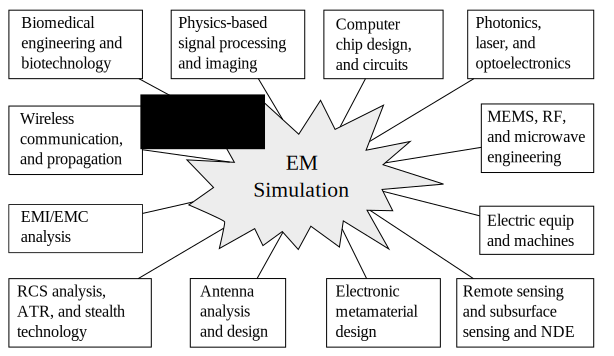
\includegraphics[scale=0.5]{./img/EM_simulation_applications.pdf}
\caption{Maxwell equations by the hand of numerical methods have the power to impact many scientific and technological areas. Taken from Jin et al \cite{Jin2010}}.
\label{fig:simulation_areas}
\end{figure}

In the context of Universidad EAFIT, and specifically of Engineering Physics, we see a growing research background in computational physics that goes from modeling seismic waves \cite{Guarin2012}, and resonant modes in musical instruments \cite{Rodriguez2012}; passing through quantum mechanics like relativistic phenomena in graphene \cite{Villegas2011}, and quantum potential wells and crystals \cite{Echeverri2011}; to finally address a computational module for digital holography and speckle \cite{Sierra2010}, and research on Plane Wave Methods for calculation of bandgap structures in photonic crystals \cite{Loaiza2011}. It can be stated that this trend in numerical methods applied to crystal-like materials has been embraced and supported by the Computational and Theoretical Physics Research Initiative of engineering physics students (\href{https://sites.google.com/site/fisicatyc/home}{SFTyC}). This work expands and continues the initiative towards strengthening undergraduate research and software development abilities. 

% There is also a backgrownd in simulation of solid state physics problems in my context. (Reference Edward, and Yefferson). It is cool that people in college understand about programming, numerical methods and their implementation.

%PCs are a good candidate for laser fabrication because point defects in the structure allows localized modes 

%Mention: 
%* The importance of research in photonic crystals (check)
%* Nice technological applications of photonic crystals (close)
%* Work of the theoretical and computational physics  research initiative, and past work on simulation of Quantum Wells and periodic structures... even if we didn't conclude great achievements (check)
%* Importance of developing abilities in computational physics
\pagebreak

\chapter{Electromagnetic waves in periodic media}
\label{ch:Electromagnetic waves in periodic media}

This chapter focuses on basic concepts and principles related to electromagnetic fields and waves based on Maxwell's equations. More over, some emphasis will be taken on stating these equations as a linear Hermitian Eigenvalue problem that has many common points with the Schr\"odinger equation and its application to crystals in the field of Solid State Physics \cite{Kittel2005}. 
In this way, propagation of light in a photonic crystal can be defined using linear operators acting over wave functions that are solution to a given eigenvalue problem.  Periodicity is then invoked by means of discrete translational symmetry operators, and their associated phase shift eigenvalue. 

\section{Maxwell equations}

The macroscopic behavior of electromagnetism, including propagation of light in Photonic Crystals (PCs) are governed by \textbf{Maxwell equations}. Maxwell's equations are four (vectorial) equations that relate the electric and magnetic fields to their respective sources, i.e. electric charges and currents. They were established by James Clerk Maxwell (1831-1879) based on experimental discoveries of Andr\'e-Marie Ampere (1775-1836) and Michael Faraday (1791-1867), and a law of electricity made by Carl Friederich Gauss (1777-1855) \cite{Jin2010}.

These equations are herein expressed in both their Integral and Differential forms. Further information on their derivation can be found in classical textbooks on Electromagnetism (e.g. \cite{Jackson1998}). 

Maxwell equations in integral form are closer to the fundamental postulates that inspired them and use integration of the fields over volumes surfaces and closed paths to relate fields and their sources. They are: 
\begin{align}
&\oint_C \mathbf{E}\cdot d\mathbf{l} = -\frac{d}{dt}\int_S \mathbf{B}\cdot d\mathbf{S} &\mbox{(Faraday)}\\
&\oint_C \mathbf{H}\cdot d\mathbf{l} = \frac{d}{dt}\int_S \mathbf{D}\cdot d\mathbf{S} + \int_S \mathbf{J}\cdot d\mathbf{S} &\mbox{(Ampere-Maxwell)}\\
&\int_S \mathbf{D}\cdot d\mathbf{S} = \int_V \rho dV &\mbox{(Gauss)} \label{eq:Gauss}\\
&\int_S \mathbf{B}\cdot d\mathbf{S} = 0 &\mbox{(Gauss for magnetism)},
\end{align}

In differential form Maxwell's equations are as follows
\begin{align}
&\nabla\times \mathbf{E} = - \frac{\partial \mathbf{B}}{\partial t} &\mbox{(Faraday)} \label{eq:diff_Faraday}\\
&\nabla\times \mathbf{H} =  \frac{\partial \mathbf{D}}{\partial t} + \mathbf{J} &\mbox{(Ampere-Maxwell)} \label{eq:diff_Ampere}\\
&\nabla\cdot \mathbf{D} = \rho &\mbox{(Gauss)} \label{eq:diff_Gauss}\\
&\nabla\cdot \mathbf{B} = 0 &\mbox{(Gauss for magnetism)} \label{eq:diff_Gauss2}\\
&\nabla\cdot \mathbf{J} = -\frac{\partial \rho}{\partial t} &\mbox{(Continuity)}, \label{eq:diff_cont}
\end{align}

In both set of equation we have
\begin{itemize}
\item $\mathbf{E}$: Electric field intensity (volts/meter),
\item $\mathbf{D}$: Electric flux density (coulombs/meter$^2$),
\item $\mathbf{H}$: Magnetic field intensity (amperes/meter),
\item $\mathbf{B}$: Magnetic flux density (webers/meter),
\item $\mathbf{J}$: Electric current density (amperes/meter$^2$),
\item $\rho$: Electric charge density (coulombs/meter$^3$).
\end{itemize}

Even though they may appear in this document it is important to say that in the implementation and simulations no current or charge densities are considered so $\rho = 0$ and $\mathbf{J} =0$, what is common for the case of electromagnetic waves far away from the sources.
Being structures from which light must propagate, Photonic Crystals are made of dielectric, translucent  materials that have a given permeability or dielectric constant called $\epsilon$. When fields propagate through dielectric media, the dielectric gets electrically polarized and this affects the field. A polarization field known as polarization vector $\mathbf{P}$ appears and then the electric flux density is defined for a material with dielectric constant $\epsilon$.  A similar phenomenon happens with magnetic fields and materials that get magnetized, and an equivalent constitutive relation is constructed but now with the parameter $\mu$ or permeability.
So, the two constitutive relations in EM are:
\begin{align}
&\mathbf{D} = \epsilon_0 \mathbf{E} + \mathbf{P}\\
&\mathbf{B} = \mu_0  \mathbf{H} + \mathbf{M},
\end{align}
where $\mathbf{P}$ is the polarization vector that tell us information about the response of the material to the external field due to orientation of the molecules inside of it, and $\mathbf{M}$ is the magnetization vector that is the analogous of the polarization for the magnetic case. If the fields are small enough the behavior of the material is linear and we can express the polarization and magnetization vectors as linear functions of $\mathbf{E}$ and $\mathbf{H}$
\begin{align}
&\mathbf{D} = \bar{\bar{\epsilon}} \cdot \mathbf{E}\\
&\mathbf{B} = \bar{\bar{\mu}} \cdot \mathbf{H},
\end{align}
where the double bar refers to a second order tensor, and $\cdot$ is a tensor-vector product. A tensorial formulation is necessary if the material is anisotropic, this is, if its properties vary depending of the direction from where you look at them. If the material is isotropic (its the same from every angle), then we can assume $\bar{\bar{\epsilon}}$ and $\bar{\bar{\mu}}$ as scalars. Thorough the following chapters, and in the implementation of the software, these two quantities are assumed as scalars.

Another important fact to notice is that PC's do not generally involve magnetic constitutive materials, so from here on we will assume no magnetization $\mathbf{M} = 0$, $\mu = \mu_0$. 

\section{Wave equation for electric fields}

As we can see in equations \ref{eq:diff_Faraday} \ref{eq:diff_Ampere} the electric and magnetic fields are coupled. One of the great achievements from Maxwell's work on stating these equations, was the discovery that the right operations for the uncoupling of these equations leads to a wave equation that explains electromagnetic radiation.

If we take the curl to \eqref{eq:diff_Faraday}, we get
\[ \nabla\times\nabla\times\mathbf{E} = -\frac{\partial}{\partial t} \nabla\times \mathbf{B} = -\frac{\partial}{\partial t} \nabla\times (\bar{\bar{\mu}} \cdot \mathbf{H}) \enspace , \]
assuming a (piece wise\footnote{Because in our formulation of the Finite Element we need the functions to be smooth (in the first derivative) only inside elements}) homogeneous material,
\begin{align*}
\nabla\times\nabla\times \mathbf{E} = - \frac{\partial}{\partial t} \nabla\times \mathbf{B} &= \- \frac{\partial}{\partial t} ( \bar{\bar{\mu}}\cdot \nabla\times \mathbf{H})\\
&= -\frac{\partial}{\partial t} \left( \bar{\bar{\mu}}\cdot \left[ \frac{\partial \mathbf{D}}{\partial t} + \mathbf{J}\right] \right)\enspace ,
\end{align*}
and if the polarization and magnetization do not vary with time --there is not hysteresis-- we have:
\begin{align}
&\nabla\times\nabla\times \mathbf{E} = -\bar{\bar{\mu}}\cdot \left[ \frac{\partial^2 \mathbf{D}}{\partial t^2} + \frac{\partial \mathbf{J}}{\partial t} \right] \nonumber \\
&\nabla\times\nabla\times \mathbf{E} = -\bar{\bar{\mu}}\cdot \left[ \bar{\bar{\epsilon}}\cdot\frac{\partial^2 \mathbf{E}}{\partial t^2} + \frac{\partial \mathbf{J}}{\partial t} \right] \label{eq:E-wave-loads} \enspace .
\end{align}
Similarly, if we take the curl to \eqref{eq:diff_Ampere}, under the same assumptions we get
\begin{align*}
\nabla\times\nabla\times \mathbf{H} &= \frac{\partial \nabla\times \mathbf{D}}{\partial t} + \nabla\times \mathbf{J}\\
&= \frac{\partial \nabla\times (\bar{\bar{\epsilon}}\cdot\mathbf{E})}{\partial t} + \nabla\times \mathbf{J}\\
&= \frac{\partial  \bar{\bar{\epsilon}}\cdot\nabla\times\mathbf{E}}{\partial t} + \nabla\times \mathbf{J}\\
&= \frac{\partial  \bar{\bar{\epsilon}}\cdot\left(-\frac{\partial \mathbf{B}}{\partial t}\right)}{\partial t} + \nabla\times \mathbf{J} \enspace ,
\end{align*}
and thus
\begin{align}
&\nabla\times\nabla\times \mathbf{H} = -\bar{\bar{\epsilon}}\cdot  \frac{\partial^2 \mathbf{B}}{\partial t^2} +  \nabla\times\mathbf{J} \nonumber \\
&\nabla\times\nabla\times \mathbf{H} = -\bar{\bar{\epsilon}}\cdot  \bar{\bar{\mu}}\cdot\frac{\partial^2 \mathbf{H}}{\partial t^2} + \nabla\times\mathbf{J} \label{eq:H-wave-loads} \enspace .
\end{align}
If we apply the vector identity $\nabla\times\nabla\times \mathbf{A} = \nabla(\nabla\cdot\mathbf{A}) - \nabla^2 \mathbf{A}$, and assume that we do not have electrical charges we can rewrite \eqref{eq:E-wave-loads} and \eqref{eq:H-wave-loads} as
\begin{align}
&\nabla^2 \mathbf{E} = \bar{\bar{\mu}}\cdot\bar{\bar{\epsilon}}\cdot \frac{\partial^2 \mathbf{E}}{\partial t^2} - \bar{\bar{\mu}}\cdot \frac{\partial \mathbf{J}}{\partial t} \\
&\nabla^2 \mathbf{H} = \bar{\bar{\epsilon}}\cdot\bar{\bar{\mu}}\cdot \frac{\partial^2 \mathbf{H}}{\partial t^2} - \nabla\times \mathbf{J}
\end{align}


Neglecting terms $\frac{\partial \mathbf{J}}{\partial t}$ and $\nabla\times \mathbf{J}$ --the source terms in the equations-- and assuming isotropy we get the well known expressions:
\begin{align}
&\left(\nabla^2 - \mu\epsilon \frac{\partial^2}{\partial t^2} \right) \mathbf{E} = \mathbf{0} \label{eq:E-wave-homo}\\
&\left(\nabla^2 - \mu\epsilon \frac{\partial^2}{\partial t^2} \right) \mathbf{H} = \mathbf{0} \label{eq:H-wave-homo} \enspace ,
\end{align}
that are vectorial wave equations with phase speed $c = \sqrt{\epsilon \mu}$. 

This form of \eqref{eq:E-wave-loads} is relevant for us because the program is currently based on this approximation. This particular topic will be treated furthermore in the implementation section \ref{sec:Implementation}.


\section{Time harmonic fields, reciprocal space and Fourier transform}

Linearity of Maxwell equations, and a restriction to time harmonic variations permits the separation of time and spatial dependencies in the form:

$$ \mathbf{E}(\mathbf{r},t) =\mathbf{E}(\mathbf{r})e^{-i\omega t} $$

This is known as a phasorial notation, and from here on, when dealing with time harmonic fields we will be interested only on the unknown phasor function $\mathbf{E}(\mathbf{r})$ which will represent the field distribution at a fixed time.

Considering a single harmonic wave propagating with angular frequency $\omega$ we get:
\begin{align}
&\nabla\times\nabla\times \mathbf{E} = -\omega^2\bar{\bar{\mu}}\cdot\bar{\bar{\epsilon}}\cdot \mathbf{E} - i\omega\bar{\bar{\mu}}\cdot  \mathbf{J} \label{eq:E-wave-harmonic}\\
&\nabla\times\nabla\times \mathbf{H} = -\omega^2\bar{\bar{\epsilon}}\cdot\bar{\bar{\mu}}\cdot \mathbf{H} + \nabla\times \mathbf{J} \label{eq:H-wave-harmonic} \enspace ,
\end{align}
These are the expressions for the frequency domain. The following relations are useful if the reader is more used to transmission line notation, and one is interested in impedance and wave numbers:

\begin{align}
&\bar{\bar{\mu}} = \mu_0\bar{\bar{\mu_r}}\\
&\bar{\bar{\epsilon}} = \epsilon_0\bar{\bar{\epsilon_r}}\\
&\mu_0 =\sqrt{\mu_0\epsilon_0}\sqrt{\frac{\mu_0}{\epsilon_0}}\\
&k_0 = \omega\sqrt{\mu_0\epsilon_0}\\
&Z_0 = \sqrt{\frac{\mu_0}{\epsilon_0}}\\
&c = \frac{1}{\sqrt{\mu_0\epsilon_0}}
\end{align}

where $\bar{\bar{\mu_r}}$,$\bar{\bar{\epsilon_r}}$  are the relative permeability and permitivity, respectively, $k_0$, $Z_0$, and $c$ are the free space wave number intrinsic impedance, and speed of light in free space. Using this we get:

\begin{align}
&\bar{\bar{\mu_r}}^{-1}\nabla\times\nabla\times \mathbf{E} = -\omega^2\mu_0\epsilon_0\bar{\bar{\epsilon_r}}\cdot \mathbf{E} - i\omega\mu_0 \mathbf{J} \\
&\bar{\bar{\mu_r}}^{-1}\nabla\times\nabla\times \mathbf{E} = k_0^{2}\bar{\bar{\epsilon_r}}\cdot \mathbf{E} - ik_0Z_0 \mathbf{J} \label{eq:E-wave-harmonic2}
\end{align}

And we actually work with either of these equations:

\begin{align}
&\dfrac{1}{\mu_r}\nabla^2 \mathbf{E} = -\omega^2\mu_0\epsilon_0\epsilon_r \mathbf{E} \\
&\frac{1}{\mu_r}\nabla^2 \mathbf{E} = k_0^{2}\epsilon_r \mathbf{E} \label{eq:E-wave-harmonic3}
\end{align}

\section{Electromagnetism as an eigenvalue problem}

The current section treats the harmonic wave equation in a formalism similar to that of quantum mechanics. It might be seen as a sumarized version of the treatment of Joannopoulos \cite{Joannopoulos2008}, and Johnson\cite{StevenJohnson2001}. Treating the equation like that will help us understand interesting qualities of electric fields and explain how they are related to the properties and geometry of the domain.

Going back to equation \ref{eq:E-wave-harmonic3}, we can see that the form of the equation is one of a eigenvalue problem. Where a series of operations on a function $\mathbf{E}$ (eigenfunction or eigenvector) gives us the same function multiplied by a constant scalar (eigenvalue).
In this case we will label the operator acting on $\mathbf{E}$ as $\hat{\Theta}$ in order to make the equation look like a simpler-looking eigenvalue problem:

\begin{equation}
\hat{\Theta}\mathbf{E} = \left(\frac{\omega}{c}\right)^2\mathbf{E}
\label{eq:simple_eigproblem}
\end{equation} 

Where:

\begin{equation}
\hat{\Theta}\mathbf{E}\triangleq \bar{\bar{\mu_r}}^{-1}\nabla\times\nabla\times \mathbf{E}
\end{equation}

Here the eigenvectors or phasors $\mathbf{E}$ represent spatial patterns of the harmonic modes, and eigenvalues $ \left( \frac{\omega}{c}\right)^2$ give information about the frequency $\omega$ (and thus wave number $k_0$) of such modes.
\subsection{Hermiticity}
As in Quantum Mechanics with the Hamiltonian, some key properties of the eigenfunctions that satisfy equation \ref{eq:simple_eigproblem} are \footnote{This proposition holds if we are not considering lossy materials, where the properties are treated as complex valued tensor and then the operator is no longer Hermitian.}:
\begin{itemize}
\item Have real eigenvalues,
\item are orthogonal,
\item can be obtained by a variational principle
\item and can be catalogued by symmetry properties .
\end{itemize}

All of these properties rely on the fact that the linear operator is from a kind known as \textbf{Hermitian operator}. To understand why $\hat{\Theta}$ is Hermitian we need first to understand the inner product of two wavefunctions $\mathbf{F(r)}$ and $\mathbf{G(r)}$:

\begin{equation}
\left( \mathbf{F(r)},\mathbf{G(r)}\right)  \triangleq
\int \mathbf{F^*(r)}\cdot \mathbf{G(r)}
\label{eq:inner_prod}
\end{equation}

where $^*$ denotes complex conjugation. From definition \ref{eq:inner_prod} we can see that:
$\left(\mathbf{F},\mathbf{G}\right) =  \left(\mathbf{G},\mathbf{F}\right)^*$
 for and $\mathbf{F}$ and $\mathbf{G}$. Also, $\left(\mathbf{F},\mathbf{F}\right)$ is always real and non-negative, and $\left(\mathbf{F},\mathbf{F}\right)$ is known as the $L^2$ norm of $\mathbf{F}$. A normalized wavefunction is one where 
 $\left(\mathbf{F},\mathbf{F}\right)=1$.

Having defined an inner product for two wavefunctions, we say that any operator $\hat{\Theta}$ is \textbf{Hermitian} if $\left(\mathbf{F},\hat{\Theta}\mathbf{G}\right) = \left(\hat{\Theta}\mathbf{F},\mathbf{G}\right)$
for any fields $\mathbf{F}$ and $\mathbf{G}$. 

Using this, we can check that the operator in equation \ref{eq:E-wave-harmonic2} is Hermitian and derive nice properties around that conclusion:

\begin{align}
\left(\mathbf{F},\hat{\Theta}\mathbf{G}\right) &=
\int \mathbf{F^*}\cdot \frac{1}{\bar{\bar{\mu_r}}}\nabla\times\nabla\times \mathbf{G}\\
& = \int \left(\nabla\times\mathbf{F}\right)^*\cdot
	\frac{1}{\bar{\bar{\mu_r}}}\left(\nabla\times\mathbf{G}
	\right)+ \int \nabla\cdot\left( \mathbf{F} \times \frac{1}{\bar{\bar{\mu_r}}}\nabla\times\mathbf{G} \right)\\
&= \int \left[\nabla\times \left(\frac{1}{\bar{\bar{\mu_r}}}\nabla\times\mathbf{F}\right)\right]^*
\cdot\mathbf{G} + 
\int \nabla\cdot\left(\nabla\times\mathbf{F} \times \frac{1}{\bar{\bar{\mu_r}}}\nabla\times\mathbf{G} \right)+\int \nabla\cdot\left( \mathbf{F} \times \frac{1}{\bar{\bar{\mu_r}}}\nabla\times\mathbf{G} \right) \\
& = \int \left[\nabla\times \left(\frac{1}{\bar{\bar{\mu_r}}}\nabla\times\mathbf{F}\right)\right]^*
\cdot\mathbf{G} \\
&= \left(\hat{\Theta}\mathbf{F},\mathbf{G}\right)
\label{eq:hermiticity_proof}
\end{align}

Here the vector cross product identity\footnote{$\nabla \cdot \left(\mathbf{A}\times \mathbf{B} \right) = \mathbf{B}\cdot\left(\nabla \times \mathbf{A} \right) - \mathbf{A}\cdot\left(\nabla \times \mathbf{B} \right)$ With $\mathbf{A} = \mathbf{F}$ and $\mathbf{B} =\nabla\times\mathbf{G}$, first and then $\mathbf{A} = \nabla\times\mathbf{F}$ and $\mathbf{B} =\mathbf{G}$} is used twice and surface terms that derive from using the Divergence Theorem are neglected.

The importance of knowing that the operator in the left side of \ref{eq:E-wave-harmonic2} is hermitian resides in the fact that Hermitian operators have real numbers as eigenvalues.
This can be seen by taking the inner product $\left(\mathbf{E},\hat{\Theta}\mathbf{E}\right)$ and observing  that operation of $\hat{\Theta}$ on one of its eigenvectors $\mathbf{E}$ produces the same eigenvector multiplied by the eigenvalue as shown in \ref{eq:simple_eigproblem}. Then:
$$
\left(\mathbf{E},\hat{\Theta}\mathbf{E}\right) = \left(\frac{\omega}{c}\right)^2\left(\mathbf{E},\mathbf{E}\right)
$$
Given that $\left(\mathbf{E},\mathbf{E}\right)$ is real, as we mentioned before, when taking the complex conjugate 
of that product we have:
$$
\left(\mathbf{E},\hat{\Theta}\mathbf{E}\right)^* = \left(\frac{\omega^2}{c^2}\right)^*\left(\mathbf{E},\mathbf{E}\right)
$$
and being Hermitian: 
\begin{align*}
\left(\mathbf{E},\hat{\Theta}\mathbf{E}\right)^* &= \left(\mathbf{E},\hat{\Theta}\mathbf{E}\right)^* \\
\left(\frac{\omega^2}{c^2}\right)^*\left(\mathbf{E},\mathbf{E}\right) &= \left(\frac{\omega^2}{c^2}\right)\left(\mathbf{E},\mathbf{E}\right)
\end{align*}

Speed of light $c$ is real, so $\omega^2 = \left(\omega^2\right)^*$ must be real.

\subsection{Symmetry groups}

As in Quantum Mechanics and any other eigen-problems, we must introduce the concept of orthogonality in order to understand other operations.
We say that two wavevectors are \textbf{orthogonal} if $\left(\mathbf{E},\mathbf{E}\right) = 0$, and this happens whenever they have different frequencies. This can be seen as a product of Hermiticity of operator $\hat{\Theta}$ by the following operation on two different modes $\mathbf{E}_1$ and $\mathbf{E}_2$:
\begin{align*}
c^2\left(\mathbf{E}_2,\hat{\Theta}\mathbf{E}_1\right) &=
c^2\left(\hat{\Theta}\mathbf{E}_2,\mathbf{E}_1\right) \\
\omega_1^2\left(\mathbf{E}_2,\mathbf{E}_1\right) &= \omega_2^2\left(\mathbf{E}_2,\mathbf{E}_1\right) \\
\left(\omega_1^2-\omega_2^2\right) \left(\mathbf{E}_2,\mathbf{E}_1\right) &= 0
\end{align*}
From this one can see that if two eigenfunctions have different frequencies ($\omega_1^2-\omega_2^2\neq 0$) then $\left(\mathbf{E},\mathbf{E}\right) = 0$
must be true and they are orthogonal.
Now, if $\left(\omega_1^2-\omega_2^2\right) = 0$ then $\mathbf{E}_1$ and $\mathbf{E}_2$ are not necessarily orthogonal, and the value is known as a \textbf{degenerate} frequency because there is more than one state or wavefunction with eigenvalue $\left(\frac{\omega^2}{c^2}\right)$. In this section we will see that degeneracy is related with symmetries of the domain, and that will be useful for the solution of periodic problems.  

Symmetry operations are operations that do not transform the wavefunction of a mode. Symmetries of a problem are such that if a symmetry operation is applied to the wavefunction, it remains the same but multiplied by a scalar. This is called being invariant under the operation.
So rotation, inversion, and reflections, are common symmetry operations that can be applied to systems that are symmetric under rotation, inversion and reflection, respectively. 
Probably the most immediate symmetry operation one can think of is the identity operation:
$\hat{E}\mathbf{E(r)} = \mathbf{E(r)}$, that transform a system into itself.

Another interesting operation is that of Inversion ($\hat{O_I}$), which takes a function $\mathbf{E(r)}$ and inverts its argument: $\hat{O_I}\mathbf{E(r)} = \mathbf{E(-r)}$. If $\mathbf{E(-r)}=\mathbf{E(r)}$ we say that the mode is invariant under inversion, or invertible.
Finally, the translation operator is one where the argument gets shifted in space by a given displacement $\mathbf{d}$: $\hat{T}_d\mathbf{E(r)} = \mathbf{E(r-d)}$. 
One function that is invariant over translation operations is a plane wave like $e^{ikz}$, because operation of $\hat{T}$ over the planewave gives the same wavefunction by a scalar $e^{-ik\mathbf{d}}$:
$$\hat{T}e^{ikz} = e^{ik(z-\mathbf{d})} = e^{-ik\mathbf{d}}e^{ikz}$$
We can see here that this is an eigenvalue problem with eigenfunctions of the form  $e^{ikz}$ and complex eigenvalues $e^{-ik\mathbf{d}}$.
Now, operators can act on other operators, and they can also be invariant under symmetry operations. If we have an operator $\hat{\Theta}$ whose intrinsic medium properties are characterized by $\bar{\bar{\epsilon}}$ and $\bar{\bar{\mu}}$, and those properties are homogeneous in space, we will be acting on a system with translational symmetry. That is, the operator is the same at different points in space.
So, if we have a wave function $\mathbf{E(r)}$ displace it with $\hat{T_d}$, then act on it with $\hat{\Theta}$ and displace it back with an inverted translation operator $\hat{T_d}^{-1}$ we will get the same result as if only $\hat{\Theta}$ was used:

\begin{align*}
\hat{\Theta}\mathbf{E(r)} &= \hat{T_d}^{-1}\hat{\Theta}\hat{T_d}\mathbf{E(r)}\\
\hat{\Theta} &= \hat{T_d}^{-1}\hat{\Theta}\hat{T_d}
\end{align*}

Whenever that happens with operators, we can write it in the form: \[\hat{T_d}\hat{\Theta}-\hat{\Theta}\hat{T_d}=0\]
and bring the definition of \textbf{commutator} between two operators as in Quantum Mechanics: 
\begin{equation}
\left[\hat{A},\hat{B}\right] \triangleq \hat{A}\hat{B}-\hat{B}\hat{A}
\label{eq:commutator}
\end{equation}
If $\left[\hat{A},\hat{B}\right] = 0$ we say that $\hat{\Theta}$ commutes with $\hat{T_d}$, and that implies that that there are wavefunctions common to both.
This is useful because sometimes eigenvalues and eigenfunctions of simple symmetry operators are easier to determine than those of $\hat{\Theta}$.  
The set of symmetry operators that commute with $\hat{\Theta}$ forms the symmetry group of the problem.  
The fact that plane wave solutions are a solution of the homogeneous isotropic wave equation problem is a consequence of them being solution to a continuous translational symmetry operation that commutes with the operator of the problem.
``When one has commuting operators, one can choose simultaneous eiigenvectors of both operators'' \cite	{Joannopoulos2008}

\subsection{Discrete translational symmetries}
Photonic crystals, like crystals of atoms or molecules do not have continuous translational symmetry, instead, they have discrete translational symmetry \cite{Joannopoulos2008}. This means that the ruling operator for the field inside a photonic crystal is invariant only for certain translation operations, specifically those in which the distance of translation $r'$ is multiple of some fixed length that we will call a \textbf{primitive lattice vector}.

\begin{figure}
\centering
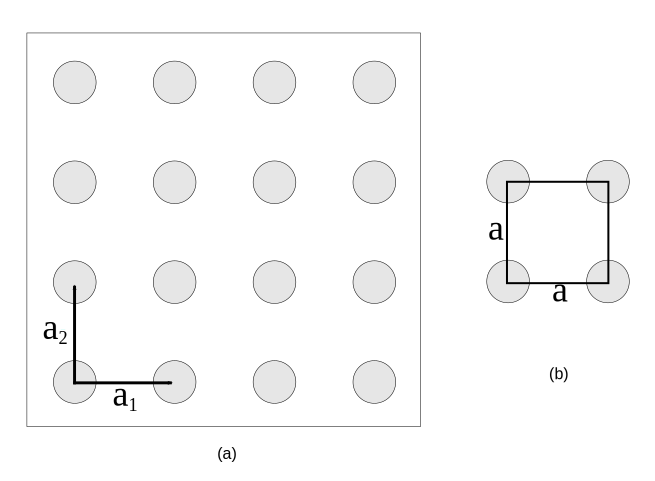
\includegraphics[scale=0.5]{./img/squarel.pdf}
\caption{Illustration of a bi dimensional point lattice: a) Section of a square lattice with primitive lattice vectors $a_1$ and $a_2$ b)  and one of the possible correspondent unitary cells where corners of four points are shared by one cell. Taken with permission from \cite{Guarin2012}.}
\label{fig:sq_lat_fig}
\end{figure}

So, if we have a 2D lattice of dielectric rods in air like in figure \ref{fig:sq_lat_fig} where the dielectric constant is a periodic function of space $\epsilon = \epsilon_0\epsilon_r(r)$\footnote{In which $\epsilon$ for air is $\epsilon(r) = \epsilon_0$ and inside the rod we have some positive realizable value $\epsilon_r$. And $r= x\hat{x}+y\hat{y}$}, then following what we learn in a solid state course we can define the crystal as a base (for example one rod) and a lattice. Which is the set of all discrete translation operations that are a linear combination of  multiples of the two primitive translation lattice vectors $a_1$ and $a_2$\cite{Kittel2005}. Or in a mathematical notation:
\begin{align}
&r' = r+u_1a_1+u_2a_2\\
& \hat{T}_{r'}\mathbf{E(r)} = \mathbf{R(r-r')} 
\label{eq:discrete_periodic}
\end{align}
where $u_1$ and $u_2$ are integers. If $\mathbf{E}$ is a plane wave, then we have 
\begin{align*}
\hat{T}_{r'}e^{i\vec{k}\cdot r} &= e^{i\vec{k}\cdot (r-r')}\\
\hat{T}_{r'}e^{i\vec{k}\cdot r} &= e^{i\vec{k}\cdot r} e^{i\vec{k}\cdot r'}
\end{align*}
with $\vec{k} = \vec{k}_x+\vec{k}_y$ as the wave vector with two components.
\begin{align}
\hat{T}_{r'}e^{i\vec{k}\cdot r} &= e^{i\vec{k}\cdot r} e^{i\vec{k}_x u_1a_1}e^{i\vec{k}_x u_2a_2}\label{eq:discrete_periodicity}
\end{align}

Now, \ref{eq:discrete_periodicity} does not immediately satisfy the form of equation \ref{eq:discrete_periodic} and we don't have an eigenfunction of the lattice. In order to get a solution that is invariant under discrete translations $r'$, the factor $e^{i\vec{k}\cdot r'}$ must be equal to 1, and this is obtained when one of two things happen, either $\vec{k}\cdot r' = 0$ or $\vec{k}\cdot r' = 2\pi n$ for $n = 1,2,3...$.
The first, is a trivial solution where there is no wave, on the other hand, the second is valid for any combination of $\vec{k_x}$ and $\vec{k_y}$ that happens to satisfy $\vec{k_x} = \frac{2\pi m}{a_1}$ and $\vec{k_y} = \frac{2\pi m}{a_2}$.  The minimal quantities $b_1 = \frac{2\pi}{a_1}$ and $b_2 = \frac{2\pi}{a_2}$ are known as the primitive vectors of the reciprocal lattice, and the linear combination of integer multiples of them form the reciprocal lattice (shown in figure ), which is the set of all arbitrary reciprocal lattice vectors defined by:

\[G = v_1b_1+v_2b_2\]

\begin{figure}
\centering
\includegraphics[scale=.5]{./img/squarer.pdf}
\caption{Illustration of a bi dimensional point lattice in the reciprocal domain: a) Section of a square lattice with primitive reciprocal lattice vectors $b_1$ and $b_2$ b)  and a reciprocal unitary cells best known as the first Brillouin zone. Taken with permission from \cite{Guarin2012}.}
\end{figure}

The nice thing about reciprocal lattice vectors is that a given wave vector $\vec{k}$ will have an indistinguishable effect on the wave from a wave vector $\vec{k} + G$ that is translated by a reciprocal lattice vector.  And remembering that $\hat{T_d}$ commutes with $\hat{\Theta}$, a general solution for $\mathbf{E}$ can be arranged by having a linear combination of the functions with different $\vec{k} + G$ that are solution to equation \ref{eq:discrete_periodic}. This is done as follows:

\begin{align*}
\mathbf{E(r)}_{\vec{k}} &= \sum_{m,n}C_{m,n}e^{i(\vec{k}+G_{m,n})\cdot r}\\
\mathbf{E(x,y)}_{k_x,k_y} &= \sum_{m,n}C_{m,n}e^{i(\vec{k}_x + mb_1)x}e^{i(\vec{k}_y + mb_2)y}\\
\mathbf{E(x,y)}_{k_x,k_y} &= e^{i\vec{k}_x x}e^{i\vec{k}_y y}\sum_{m,n}C_{m,n}e^{imb_1x}e^{imb_2y}\\
\mathbf{E(r)}_{\vec{k}} &= e^{i\vec{k}\cdot r} \mathbf{u}_{\vec{k}}(r)
\end{align*}

Where $\mathbf{u}_{\vec{k}}(r)$ is by definition a bi-periodic function in $r$ that satisfies  $\mathbf{u}_{\vec{k}}(r+r') = \mathbf{u}_{\vec{k}}(r)$ for a given $\vec{k}$.This result is commonly known as Bloch's Theorem, in solid state physics, and in mechanics as Floquet's. $C_{m,n}$ are expansion coefficients to be solved by explicit solution and are the key for the formulation of the Plane Wave Expansion (PWE) method \cite{Loaiza2011, Joannopoulos2008, StevenG, Johnson2001}. We however are not interested in $C_{m,n}$, because we are not solving for plane waves. Instead we will use this as a boundary condition by identifying how is the field after a translation of an arbitrary lattice vector $R$:

\begin{align}
\mathbf{E(r+R)}_{\vec{k}} &= e^{i\vec{k}\cdot (r+R)} \mathbf{u}_{\vec{k}}(r+R)\\
\mathbf{E(r+R)}_{\vec{k}} &= e^{i\vec{k}\cdot R}e^{i\vec{k}\cdot r} \mathbf{u}_{\vec{k}}(r)\\
\mathbf{E(r+R)}_{\vec{k}} &= e^{i\vec{k}\cdot R}\mathbf{E(r)}_{\vec{k}}
\end{align}

We now know that if $R$ is a lattice vector like $r'$, the solution of the field at that point will be exactly the same than the solution of the filed in the point before the translation multiplied by a complex factor $e^{i\vec{k}\cdot R}$. So given a known wave vector $\vec{k}$ and the solution of every point inside the base, or unitary cell, one can know the value of $\mathbf{E}$ everywhere. This is because the boundaries of a unit cell are separated by a distance that is either $a_1$ in $x$ or $a_2$ in $y$. Details about how to implement this condition in a numerical solution are given in \cite{Guarin2012}.

\subsection{Conservation of energy for waves in source less media}

We define the energy of a field $\mathbf{w}$ as its norm $||\mathbf{w}||^2 = \left(\mathbf{w},\mathbf{w}\right)$.
Conservation of energy in time in a source-less problem like that of equation \ref{eq:E-wave-loads} is obtained when $||\mathbf{w}||^2$ variation in time is zero, thus:
\begin{equation}
\frac{\partial ||\mathbf{w}||^2}{\partial t} =\frac{\partial \left(\mathbf{w},\mathbf{w}\right)}{\partial t} = \left(\dot{\mathbf{w}},\mathbf{w}\right)-\left(\mathbf{w},\dot{\mathbf{w}}\right) = \left(\hat{\Theta}\mathbf{w},\mathbf{w}\right)+\left(\mathbf{w},\hat{\Theta}\mathbf{w}\right) = \left(\hat{\Theta}\mathbf{w},\mathbf{w}\right)-\left(\hat{\Theta}\mathbf{w},\mathbf{w}\right) = 0
\end{equation}
Remembering that in a problem that is not harmonic we have $\hat{\Theta}\mathbf{E} = \frac{\partial^2 \mathbf{E}}{\partial t^2}$This means that under Hermitic operators such as $\hat{\Theta}$ the energy of the field is conserved\footnote{This expression for energy conservation holds only for cases where the operator does not change in time. A case where we have time varying material properties $\epsilon(r,t)$ can break conservation of energy if the time variation changes the norm\cite{Johnson07noteson}}.

\subsection{Energy functional of electromagnetic waves}
 
By means of the \textbf{electromagnetic variational theorem} we can formulate an energy functional to  to be minimized. This functional is defined as a normalized inner product between the function and the function multiplied by the following operator known as Rayleigh Quotient:
\begin{equation}
U_f(\mathbf{E}) \triangleq \frac{\left(\mathbf{E}, \hat{\Theta} \mathbf{E}\right)}{\left(\mathbf{E},\mathbf{E}\right)}
\label{eq:energy_functional}
\end{equation}

It is similar to other formulations used in fields like Quantum Mechanics and Classical mechanics such as expectation values, and energy Lagrangians.  The process of finding solutions that minimize such a potential is the core of what methods like Galerkin do for solving differential equations. In chapter \ref{ch:Finite_element_method} we will use a similar expression in order to solve the wave equation using Galerkin with Finite Elements.
 
\chapter{Finite element method}
\label{ch:Finite_element_method}

%El calculo variacional es una disciplina que se encarga de encontrar el minimo de un funcional. En donde un funcional es el mapeo de un espacio vectorial a los reales. Si esta es la ecuacion diferencial
%
%Lu = f
%
%Entonces el residuo es
%
%R(v) = Lv - f
%
%y si se evalua en la solucion u
%
%R(u) = 0
%
%entonces minimizar un residio no tiene gracia, porque se trata de encontrar la solucion exacta a la ecuacion diferencial. Que es lo que no sabemos hacer. Pero entonces podemos proponer minimizar un residuo promediado, p. ej., la norma del error. Entonces definimos un residuo ponderado
%
%Rp(u,v) = int(v*Lu - v*f)
%
%(weigthin se dice ponderar en espanhol). Entonces, uno propone una solucion con una forma conocida: senos y cosenos, polinomios, Gaussianas... Y encuentra la combinacion lineal de esas funciones que minimiza Rp (Y a estamos hablando de metodos aproximados para resolver la ecuacion diferencial).

The Finite Element Method approximates an integral formulation that is --in some sense-- equivalent with a differential equation. This integral (weak) formulation can be obtained from a variational principle, such as the Principle of Virtual Works, or the Integral of Action \cite{Goldstein2001}, but can also be obtained from a more general approach like the Weighted Residuals Method \cite{Zienkiewicz2005, Reddy_functional_analysis}. In the case of electromagnetic waves, we can formulate a variational principle where the functional to be minimized is the energy carried by the electric and magnetic fields defined in \ref{eq:energy_functional}. 

This project uses the Galerkin Finite Element Method to construct an approximate solution of  initial-boundary value and eigenvalue problems involving the wave equation of electromagnetic fields \ref{eq:E-wave-harmonic2}. Galerkin's method is one of these weighted residual methods in which both the weight functions and the bases for approximating the solution are defined as a linear combination of piece wise continuous polynomial functions $h$: $$u = \sum_{i=1}^Nu_ih_i.$$ Where $u_i$ are the unknown expansion coefficients and $h_i$ are the base functions. 

So if we have a general partial differential equation of the form: 
\begin{equation}
\mathcal{L}(u) = f,
\label{eq:general_form_of_DE}
\end{equation}  where $\mathcal{L}$ denotes a differential operator, $u$ denotes the unknown solution to be found and $f$ denotes source function, we can assume an approximation $u'$ of $u$ and build a residual defined as $\mathcal{R} = \mathcal{L}(u')-f$ to be minimized. What we want is to find a function $u'$ that makes $\mathcal{R}$ a minimum in an \emph{average} sense. A way to do this is to construct a functional that is defined as the integral over all space of the residual multiplied by a weighting function $w$, and then set this functional equal to zero 
\begin{equation}
\int w \mathcal{R}(u') = 0.
\end{equation}
Now depending on what bases we use to approximate $u$ and what we choose to do with the weighting functions we will get a different weighted residual method to obtain $u$. 
Galerkin's method works by defining $w$ in the same form of $u$ as shown before.

In the rest of this chapter, we will show how to apply Galerkin's Finite Element formulation to electromagnetism problems, and specifically to the time harmonic wave equation described in \ref{eq:E-wave-harmonic2} without sources. The concepts treated here are the basis of the code that has been implemented in the software platform PeyeQM that will be introduced in the following chapter.

\section{Weak formulation of the problem}

As mentioned before, in a weighted residual formulation weight functions  are used in order to minimize a functional that is stated as the integral of the operator problem over a given  simulation domain such as the one illustrated in figure \ref{fig:domain}. 

\begin{figure}[h]
\centering

\includegraphics[height=5cm]{./img/dominio.pdf}
\caption{Abstract representation of a simulation domain $\Omega$ and its boundary $\Gamma$}
\label{fig:domain}
\end{figure}

If the field we want to obtain $\mathbf{E}$ is solution to equation \ref{eq:E-wave-harmonic2}, then it must satisfy the variational form that results by multiplying \ref{eq:E-wave-harmonic2} by an arbitrary test function $\mathbf{W}$ and then integrating over $\Omega$ $\int_{\Omega} \mathbf{W} \cdot$(\ref{eq:E-wave-harmonic2}):

\begin{equation}
\int_{\Omega}\mathbf{W}\cdot\left[ \nabla\times\ \left(\mu_r^{-1}\nabla\times \mathbf{E} \right) - k_0^{2}\epsilon_r\cdot \mathbf{E}\right]= 0. \label{eq:E-wave-harmonic3} 
\end{equation}
Note that here the term $\nabla\times\ \left(\mu_r^{-1}\nabla\times \bullet \right) - k_0^{2}\epsilon_r\cdot \bullet$ stands as the operator $\mathcal{L}$ in equation \ref{eq:general_form_of_DE}. and $f=0$. Separating the two terms of this new $\mathcal{L}$ we get:
\begin{equation}
\int_{\Omega}\mathbf{W}\cdot \nabla\times\ \left(\mu_r^{-1}\nabla\times \mathbf{E} \right) -k_0^{2}\int_{\Omega}\mathbf{W}\cdot \epsilon_r\cdot \mathbf{E}= 0. \label{eq:E-wave-harmonic4} 
\end{equation}
Now, lets focus on the first integral on the left hand side of the equation. Here we will invoke the vector identity: $\mathbf{A}\cdot\nabla\times\mathbf{B} = \mathbf{B}\cdot\nabla\times\mathbf{A} - \nabla\cdot(\mathbf{A}\times\mathbf{B}.)$ 
Where $\mathbf{A}=\mathbf{W}$ and $\mathbf{B}=\epsilon_r\nabla\times \mathbf{E}$ To express it as:

\begin{equation}
\int_{\Omega}\mathbf{W}\cdot \nabla\times\ \left(\mu_r^{-1}\nabla\times \mathbf{E} \right) = \int_{\Omega} \mu_r^{-1}\nabla\times \mathbf{E}\cdot \nabla\times\mathbf{W}-\int_{\Omega}\nabla\cdot
\left(\mathbf{W}\times\mu_r^{-1}\nabla\times\mathbf{E}\right). 
\end{equation}

The Divergence Theorem allows us to transform the volume integral on the second term of the right hand side to a closed surface integral:

\begin{equation}
\int_{\Omega}\nabla\cdot
\left(\mathbf{W}\times\mu_r^{-1}\nabla\times\mathbf{E}
\right) = \oint_{\Gamma}\hat{n}\cdot
\left(\mathbf{W}\times\mu_r^{-1}\nabla\times\mathbf{E}
\right).
\end{equation}

And we will have two kinds of boundaries, Dirichlet and Neumann \cite{Garcia2011}, thus $\oint_{\Gamma} = \int_{\Gamma_D}+\int_{\Gamma_N}$. Weight functions have been conveniently chosen to be zero at Dirichlet boundaries so, $\mathbf{W}\mid_{\Gamma_D}=0$. 
One last step is to apply the triple product identity to the argument inside the Neumann integral so that:

$$\hat{n}\cdot
\left(\mathbf{W}\times\mu_r^{-1}
\nabla\times\mathbf{E}\right) =\mathbf{W} \cdot
 \left(\mu_r^{-1}\nabla\times\mathbf{E}\times\hat{n}\right) = -\mathbf{W} \cdot
 \left(\hat{n}\times\mu_r^{-1}
\nabla\times\mathbf{E}\right).$$

Substituting everything we get the form:

\begin{equation}
\int_{\Omega} \mu_r^{-1}\nabla\times \mathbf{E}\cdot \nabla\times\mathbf{W}
-k_0^{2}\mathbf{W}\cdot \epsilon_r\cdot \mathbf{E}
+ \int_{\Gamma_N} \mathbf{W} \cdot
 \left(\hat{n}\times\mu_r^{-1}
\nabla\times\mathbf{E}\right)
= 0. \label{eq:E-wave-weak} 
\end{equation}


\section{Boundary conditions}

For uniqueness of the solution and given that this is a boundary value problem, we must define how is the field or the derivative of the field at boundaries. The two conditions we come upon for defining how the system behaves at boundaries $\Gamma_D$ and $\Gamma_N$ are:
\begin{align}
\hat{n}\times\mathbf{E}&=\mathbf{P} \quad on \ \Gamma_D,\\
\hat{n}\times\left(\bar{\bar{\mu_r}}^{-1}
\nabla\times \mathbf{E}\right) &=\mathbf{K}_N \quad on \ \Gamma_N. \label{eq:BC}
\end{align}
$\mathbf{P}$ is the value for tangential electric field on Dirichlet boundaries $\Gamma_D$,  and $\mathbf{K}_N$ is a function that represents boundary sources or electric field flux on $\Gamma_N$.

Replacing equation \ref{eq:BC} in \ref{eq:E-wave-weak} we get:

\begin{equation}
\begin{array}{rcl}
\int_{\Omega} \mu_r^{-1}\nabla\times \mathbf{E}\cdot \nabla\times\mathbf{W}
-k_0^{2}\mathbf{W}\cdot\epsilon_r\cdot \mathbf{E}
&=& - \int_{\Gamma_N} \mathbf{W} \cdot\mathbf{K}_N,  \label{eq:E-wave-weak_3} 
\end{array}
\end{equation}

by using:
$$-\mathbf{W}\cdot\left(\hat{n}\times \left( \hat{n}\times 
\mathbf{E} \right)\right)  = \left(\hat{n}\times \mathbf{W}\right)\cdot\left( \hat{n}\times 
\mathbf{E} \right). $$


\section{Abstract form of the equation}

Now, in order to reduce verbosity and ease the calculations, we define a set of bi-linear operators\footnote{Which are similar to the definition of inner product made in \ref{eq:inner_prod}} who represent the integrals in \ref{eq:E-wave-weak_3}. These operators are meant to ease mathematical manipulations. Let's do some definitions first:
$\mathbb{V}$ is a vector space of square integrable functions that vanishes at Dirichlet boundaries.

$$ \mathbb{V}=\left\lbrace v\in L^2(a,b):a(v,v)<\infty\wedge v(\Gamma_D)=0\right\rbrace,$$
$$L^2 =\left\lbrace v: \Omega \rightarrow \mathbb{R}\quad such \ that\quad \int_{\Omega}v^2d\Omega =0\right\rbrace.$$ 
Operator $a$, represents the first term of the left hand side in equation \ref{eq:E-wave-weak_3}:
\begin{equation}
\begin{array}{rcl}
      a(\mathbf{W},\mathbf{E})&&:\mathbb{V}\times \mathbb{V}\rightarrow \mathbb{R},\\
      a(\mathbf{W},\mathbf{E})&&= \int\limits_{\Omega}\mu_r^{-1}\nabla\times \mathbf{E}\cdot \nabla\times\mathbf{W} d\Omega,
\label{eq:a_def}
\end{array}
\end{equation}
$b$ is the second term in the left hand side in equation \ref{eq:E-wave-weak_3}:
\begin{equation}
\begin{array}{rcl}
      m(\mathbf{W},\mathbf{E})&:\mathbb{V}\times \mathbb{V}\rightarrow \mathbb{R},\\
      m(\mathbf{W},\mathbf{E})&= \int\limits_{\Omega} k_0^{2}\mathbf{W}\cdot \epsilon_r\cdot \mathbf{E} d\Omega,
\label{eq:m_def}
\end{array}
\end{equation}
$q$ represents boundary sources.
\begin{equation}
\begin{array}{rcl}
      q(\mathbf{W})&:\mathbb{V}\rightarrow \mathbb{R},\\
      q(\mathbf{W})&=\int_{\Gamma_N} \mathbf{W} \cdot\mathbf{K}_N.
\label{eq:m_def}
\end{array}
\end{equation}
%and $f$ body source terms. In the implementation $f=0$.
%\begin{equation}
%\begin{array}{rcl}
%      f(\mathbf{W})&:\mathbb{V}\rightarrow \mathbb{R}\\
%      f(\mathbf{W})&=ik_0Z_0 \int_{\Omega} \mathbf{W}\cdot\mathbf{J}
%\label{eq:m_def}
%\end{array}
%\end{equation}
Where $\mathbf{K}_N$ is a are known boundary condition.
These operators take vectors as inputs and return scalars. Using them one can construct a form of equation \ref{eq:E-wave-weak_3} known as the abstract form:

\begin{equation}
a(\mathbf{W},\mathbf{E}) - m(\mathbf{W},\mathbf{E}) = -f(\mathbf{W})-q(\mathbf{W})
\label{eq:abstract_E_wave}.
\end{equation}

\section{Base functions and discretization}
However right now we don't have a proper Galerkin formulation because $\mathbf{E}$ is still a continuous function of all space, and thus, very hard to solve. Specifically if we are in a 2D domain where:
\[\mathbf{E}=E(x,y)_x\hat{a}_x + E(x,y)_y \hat{a}_y. \]
To have a discrete problem to solve for $\mathbf{E}$, it must be approximated, and this is done by assuming that we can write it as a linear combination of base functions. Obviously,  to have a computable problem we must take only a finite number of those base functions. What we do in FE is using piecewise polynomials as base functions, piecewise polynomials are functions that we define continuous only over disjoint finite regions of space. So a function like $\mathbf{E}$ that is continuous over all space can be split into a number $N$ of functions that each is continuous over a finite region of the domain. 
Being so, the first step is to split the domain into elements like illustrated in figure \ref{fig:disc_domain}. Each base function of the expansion will exist only within its corresponding finite region or element. With that we have
\begin{equation}
\mathbf{E} = \sum_{el=1}^{N_{el}}\mathbf{E}^{el}.
\end{equation}
Where $\mathbf{E}^{el}$ is a linear combination of interpolation functions $h_i$ who are locally continuous inside elements $el$:
\begin{equation}
\mathbf{E}^{el} = \sum_{i =1}^N E_i^{el}h_i^{el},
\end{equation}
and the values $E_i^{el}$ are the expansion coefficients that allow the functions to reach $\mathbf{E}$.
\begin{figure}
\centering
\includegraphics[scale=0.3]{./img/dominio_discreto.pdf}
\caption{Discretized domain defined by a set of elements and their nodes. Taken with permission from \cite{Guarin2012}}
\label{fig:disc_domain}
\end{figure}
Now, these functions $h_i$ can be seen as local interpolation functions of arbitrary order, and the order of the function will be proportional to the number of evaluation points in space needed to define it. The points will herein be called nodes, and they are a discrete representation of the coordinates in the domain. For higher order bases, one needs more evaluation points to define them, and because its easier to solve for lower order polynomials (fewer unknowns) we intentionally limit their order (usually to first or second order). Notice that an exact representation of $\mathbf{E}$ happens when $N\leftarrow\infty$.

\begin{figure}
\centering
\includegraphics[scale=0.5]{./img/two_dim_elem.pdf}
\caption{Three examples of commonly used two-dimensional elements. The one on the center is a 9 node quadrilateral element with a complete basis. To the left is a serendipity QUAD8 elements with 8 nodes, and to the right a 6 node triangular element.\cite{Bathe1996}}
\label{fig:2d_elem}
\end{figure}

For bi-dimensional elements like those in \ref{fig:2d_elem} one has to define one interpolation function for each node and they must be built so that on each node $i$ the function $h_i$ takes the value of 1 and zero at the rest. This is accomplished for a quadrilateral element of 4 to 9 nodes by using the functions given in table \ref{tab:int_funct}. The elements used in the software for the solution of electromagnetic fields are 8 node quadrilateral elements.
\begin{figure}
\centering
\includegraphics[scale=0.5]{./img/2D_gen_elem.pdf}
\caption{In order to ease the definition of base functions, every element is transformed to a generalized ``isoparametric element'' by means of a function $g(x,y)$ \cite{Bathe1996} so that all elements share the same base. The element on the left has an arbitrary shape and position, and by means of function $g(x,y)$ is mapped to a standard element in a domain in $r$, $s$ that goes from $-1$ to $1$. }
\end{figure}

\begin{center}
\begin{table}
\centering
    \begin{tabular}{r|c|c|c|c|c|c|}
       \multicolumn{2}{c}{~} & \multicolumn{5}{c}{Include if the node is present.}\\
       \multicolumn{1}{c}{~} & \multicolumn{1}{c|}{~} & $i=5$ & $i=6$ & $i=7$ & $i=8$ & $i=9$ \\      
    $h_1$ & $\frac{1}{4}\left(1+r\right)\left(1+s\right)$    & $-\frac{1}{2}h_5$ & ~     & ~ & $-\frac{1}{2}h_8$ & $-\frac{1}{2}h_9$ \\
    $h_2$ & $\frac{1}{4}\left(1-r\right)\left(1+s\right)$    & $-\frac{1}{2}h_5$ & $-\frac{1}{2}h_6$     &  &  & $-\frac{1}{2}h_9$ \\
    $h_3$ & $\frac{1}{4}\left(1-r\right)\left(1-s\right)$    &     & $-\frac{1}{2}h_6$ & $-\frac{1}{2}h_7$ &  & $-\frac{1}{2}h_9$ \\
    $h_4$ & $\frac{1}{4}\left(1+r\right)\left(1-s\right)$    &      &      & $-\frac{1}{2}h_7$ & $-\frac{1}{2}h_8$ & $-\frac{1}{2}h_9$ \\
    $h_5$ & $\frac{1}{2}\left(1-r^2\right)\left(1+s\right)$  &  & & &  & $-\frac{1}{2}h_9$ \\
    $h_6$ & $\frac{1}{2}\left(1-s^2\right)\left(1-r\right)$  & & &  &  & $-\frac{1}{2}h_9$ \\
    $h_7$ & $\frac{1}{2}\left(1-r^2\right)\left(1-s\right)$  & & & & &$-\frac{1}{2}h_9$ \\
    $h_8$ & $\frac{1}{2}\left(1-s^2\right)\left(1+r\right)$  & & & & & $-\frac{1}{2}h_9$ \\
    $h_9$ & $\frac{1}{2}\left(1-r^2\right)\left(1-r^2\right)$& & & & & $-\frac{1}{2}h_9$\\
    \end{tabular}
\caption{Interpolation functions of four to nine variable-number-nodes two-dimensional isoparemtric elements.}
\label{tab:int_funct}
\end{table}
\end{center}
We will proceed by presenting some notation definitions for the future development:
Lets say that the set of nodes that represent values of the field in the domain is called $\eta$. On nodes belonging to Dirichlet boundaries we will know the value of the field ($\mathbf{P}$) and it is convenient to split the set of nodes into its known and unknown elements $\eta_D\cup\eta\setminus\eta_D=\eta$.  Each physical node will contain two components of the field\footnote{In a vectorial element formulation like the one used for EM fields in our program.}, one for $x$ and the other for $y$. So the number of evaluation nodes gets doubled.

If $N$ is the total number of values:

\[N = n_x + n_y,\]

where $n_x$ and $n_y$ are the number of evaluation nodes associated to fields in $x$ and  $y$	. When programming it is convenient to distinguish where does a node belongs, so we will treat $n_x$ and $n_y$ as sets as well in order to build a notation for the sums based on  how an iterator surfs a set.


\begin{align*}
n_x &= n_x \in \eta_D + n_x \in \eta\setminus\eta_D,\\
n_y &= n_y \in \eta_D + n_y \in \eta\setminus\eta_D.
\end{align*}
If we say: $$i: n_x\in \eta_D,$$  that will mean that the iteration will occur on the indexes that belong to the set of nodes in the Dirichlet region associated to $x$ component of the field. The field for each node, for each region and and for each component can then be approximated by:

\begin{align*}
E(x,y)_x\approx \sum_{i:\ n_x \in \eta_D} h_i E_i^x+\sum_{i:\ n_x \in \eta\setminus\eta_D} h_i E_i^x,\\
E(x,y)_y\approx \sum_{i:\ n_y \in \eta_D}h_iE_i^y+
\sum_{i:\ n_x \in \eta\setminus\eta_D}h_iE_i^y.
\end{align*}
 
Left side are known values and right side unknowns.
In the same way for test functions $W$ on the boundary we have: 
\[\mathbf{W}=W(x,y)_x\hat{a}_x + W(x,y)_y \hat{a}_y, \]
\begin{align*}
W(x,y)_x\approx \sum_{i:\ n_x \in \eta_D} h_i W_i^x+\sum_{i:\ n_x \in \eta\setminus\eta_D} h_i W_i^x, \\
W(x,y)_y\approx \sum_{i:\ n_y \in \eta_D}h_iW_i^y+
\sum_{i:\ n_x \in \eta\setminus\eta_D}h_iW_i^y.
\end{align*}
Moreover $\mathbf{K}_N$ can also be interpolated if there are Neumann boundary conditions: 
%\[\mathbf{J}=J(x,y)_x\hat{a}_x + J(x,y)_y \hat{a}_y \]
%
%\begin{align*}
%J(x,y)_x\approx \sum_{i:\ n_x \in \eta_D}h_i J_i^x+\sum_{i:\ n_x \in \eta\setminus\eta_D}h_i J_i^x \\
%J(x,y)_y\approx \sum_{i:\ n_y \in \eta_D}J_i^y+
%\sum_{i:\ n_x \in \eta\setminus\eta_D}J_i^y
%\end{align*}
$$\mathbf{K}_N=K(x,y)_x\hat{a}_x + K(x,y)_y \hat{a}_y,$$
\begin{align*}
K(x,y)_x\approx \sum_{i:\ n_x \in \eta_D}h_i K_i^x+\sum_{i:\ n_x \in \eta\setminus\eta_D} 0, \\
K(x,y)_y\approx \sum_{i:\ n_y \in \eta_D}h_i K_i^y+
\sum_{i:\ n_x \in \eta\setminus\eta_D} 0.
\end{align*}

Substitution of $\mathbf{E}$ and $\mathbf{W}$, into \ref{eq:E-wave-weak_3} is a mess. To make it easier lets use the operators and their properties. To be bi linear is to be linear in both arguments, to be linear means to satisfy \href{http://en.wikipedia.org/wiki/Additive_function}{additivity} and \href{http://en.wikipedia.org/wiki/Homogeneous_function}{homogeneity}. An illustration of this:

\begin{align*}
\alpha (u+\beta v, w)&=\alpha a(u,w)+\beta a(v,w),\\
a(u,\alpha v+\beta w)&=\alpha a(u,v)+\beta a(u,w).
\end{align*}

The rotational and dot product inside the integrals defined in the abstract forms are linear. A proof for that is out of the reach of this document. 
The proof of
\[a(u,v) = a(v,u),\]
was made in equation \ref{eq:hermiticity_proof}, and a proof of
\[m(u,v) = m(v,u),\]
is obtained by assuming that $v$ and $u$ have the same base, which we did by using the Galerkin weighting.

So the following can happen:

\begin{align}
a\left(W_x,E_x\right)&=& a\left( \sum_{i:\ n_x \in \eta_D} h_i W_i^x, \sum_{j:\ n_x \in \eta_D} h_j E_j^x\right)+a\left(\sum_{i:\ n_x \in \eta\setminus\eta_D} h_i W_i^x,\sum_{j:\ n_x \in \eta\setminus\eta_D} h_j E_j^x\right)\nonumber, \\
&=&  \sum_{i:\ n_x \in \eta_D}W_i^x a\left(  h_i , \sum_{j:\ n_x \in \eta_D} h_j E_j^x\right)+\sum_{i:\ n_x \in \eta\setminus\eta_D} W_i^x a\left( h_i,\sum_{j:\ n_x \in \eta\setminus\eta_D} h_j E_j^x\right)\nonumber,\\
&=&\sum_{i:\ n_x \in \eta_D}W_i^x \sum_{j:\ n_x \in \eta_D}E_j^x a\left(  h_i ,  h_j \right)+\sum_{i:\ n_x \in \eta\setminus\eta_D} W_i^x \sum_{j:\ n_x \in \eta\setminus\eta_D}  E_j^x a\left( h_i, h_j \right)\nonumber,\\
&=& \sum_{j:\ n_x \in \eta_D} a\left(  h_i ,  h_j \right)E_j^x \sum_{i:\ n_x \in \eta_D}W_i^x+\sum_{j:\ n_x \in \eta\setminus\eta_D}   a\left( h_i, h_j \right)E_j^x\sum_{i:\ n_x \in \eta\setminus\eta_D} W_i^x \label{eq:substitution_of_app_fields_in_a}.
\end{align}

\[\sum_{j:\ n_x \in \eta_D}E_j^x = \vec{g}_j^x, \]
\[\sum_{i:\ n_x \in \eta\setminus\eta_D}W_i^x = \vec{W}^x,\]
\[\sum_{j:\ n_x \in \eta\setminus\eta_D}E_j^x = \vec{E}^x, \]
\[\vec{g}_i = \vec{g}_j^x+\vec{g}_j^y \qquad j = 1.. N, \]
$\vec{g}_j$ is a vector of size $N$ that holds values of $E$ on each Dirichlet boundary node for both $x$, and $y$ components. Vector $\hat{g}_i^y$ follows from a similar procedure on $E_y$. It is of importance to say that even though the sets defined under the summation are subsets of the set of all nodes, when programming, their associate vectors will span the whole domain. In other words this notation stands for entries to indexes to vectors that may be defined full of zeroes. Or in a different approach: $j$ in $j:\ n_x \in \eta_D$ can be indexes 1 and $N$ meaning that the first and last nodes belong to Dirichlet boundary points on $x$. All other elements of the vector are undefined and hold their initiation value zero.


Changing the indexes $i$, $j$ and using the definition of \href{http://en.wikipedia.org/wiki/Dot_product}{dot product} in a matrix notation we can translate the abstract form as:

\begin{align*}
a\left(W_x,E_x\right)=&\langle \mathbb{A}\vec{g}^x,\vec{W}^x\rangle
+\langle\mathbb{A}\vec{E}^x,\vec{W}^x\rangle . 
\end{align*}

Where $\mathbb{A}$ is a matrix whose elements contain the indexed integration over the basis functions $h_i$, and $h_j$, these are known values because we know the form of the functions and can calculate the integrals by numerical or analytic means. For the solution in the software routines we implemented numerical integration based on Gauss-Legendre quadrature as defined in \cite{Bathe1996}. 

Matrix $\mathbb{A}$ is known as the stiffness matrix in Mechanics, and here it relates to energy stored in form of electric field. Matrix $\mathbb{A}$ is built as a combination of matrices $\mathbb{A}^x$ and $\mathbb{A}^y$:
\[\mathbb{A} = \mathbb{A}^x+\mathbb{A}^y,\]
where
\[\mathbb{A}^x = \sum_{i,j}^{n_x \in \eta\setminus\eta_D} a(h_i,h_j)+\sum_{i,j}^{n_y \in \eta\setminus\eta_D} a(h_i,h_j).\]

The product $\mathbb{A}^x\vec{g}^x = \vec{d}^x$ will be called the Dirichlet vector.
\begin{align}
a\left(W_x,E_x\right)=&\langle \vec{d}^x,\vec{W}^x\rangle
+\langle\mathbb{A}^x\vec{E}^x,\vec{W}^x\rangle. \label{eq:potential_discrete} 
\end{align}

In a very similar way but now substituting the approximate functions into the kinetic operator $m(\mathbf{W},\mathbf{E})$ we get:

\begin{align}
m\left(W_x,E_x\right)=&\langle \mathbb{M}^x\vec{g}^x,\vec{W}^x\rangle
+\langle\mathbb{M}^x\vec{E}^x,\vec{W}^x\rangle\nonumber, \\
m\left(W_x,E_x\right)=&\langle \vec{b}^x,\vec{W}^x\rangle
+\langle\mathbb{M}^x\vec{E}^x,\vec{W}^x\rangle. \label{eq:kinetic_discrete}
\end{align}

With $\mathbb{M}$ as the mass matrix or inductance matrix. Being related to the time derivative of the electric field, we can associate this to energy stored in the form of magnetic fields like a sort of inductance matrix. The global mass matrix is also a combination of terms related to the degree of freedom $x$ and $y$:
\begin{align*}
\mathbb{M} &= \mathbb{M}^x+\mathbb{M}^y,\\
\mathbb{M} &= \sum_{i,j}^{n_x \in \eta\setminus\eta_D} m(h_i,h_j)+\sum_{i,j}^{n_y \in \eta\setminus\eta_D} m(h_i,h_j).
\end{align*}

And the same follows with operator $q$:

\begin{align}
q(W_x) &= \langle \vec{q}^x, \vec{W^x}\rangle \label{eq:newman},\\
\vec{q}_i^x&= \sum_{i:\ n_x \in \eta_N}\int_{\Gamma_N} h_iK_i^x \nonumber.
\end{align}

Where we introduced a subset of the set $\eta  \setminus \eta_D$ called $\eta_N$ which represents nodes on Neumann boundaries.

Substituting definitions: \ref{eq:potential_discrete}, \ref{eq:kinetic_discrete}, \ref{eq:newman}, and \ref{eq:body_source} in equation \ref{eq:abstract_E_wave}, we get:

\begin{align}
\langle\vec{d}^x,\vec{W}^x\rangle
+\langle\mathbb{A}^x\vec{E}^x,\vec{W}^x\rangle-\langle \vec{b}^x,\vec{W}^x\rangle
-\langle\mathbb{M}^x\vec{E}^x,\vec{W}^x\rangle &= -\langle \vec{q}^x, \vec{W^x}\rangle \nonumber,\\
\langle\mathbb{A}^x\vec{E}^x- \mathbb{M}^x\vec{E}^x,\vec{W}^x \rangle &=\langle \vec{b}^x-\vec{d}^x-\vec{q}^x, \vec{W}^x \rangle.
\end{align}

Being $\vec{W}^x$ an arbitrary function, the following linear system of equations appear:
\begin{equation}
\left(\mathbb{A}^x-\mathbb{M}^x\right)\vec{E}^x = \vec{b}^x-\vec{d}^x-\vec{q}^x. \label{eq:harmonic_eq_sys_x}
\end{equation}
Similarly, and following exactly the same procedure:

\begin{equation}
\left(\mathbb{A}^y-\mathbb{M}^y\right)\vec{E}^y = \vec{b}^y-\vec{d}^y-\vec{q}^y. \label{eq:harmonic_eq_sys_y}
\end{equation}


These two systems can be solved simultaneously by intercalating rows and columns of $\mathbb{A}^x$ with $\mathbb{A}^y$, and keeping the formulation as one global matrix multiplying a vector that contains values of the field in both components


\begin{equation*}
\left(\mathbb{A}-\mathbb{M}\right)\vec{E} = \vec{b}-\vec{d}-\vec{q}.
\end{equation*}

Something that is used in many references is to remove rows and columns associated to Dirichlet positions of $E$ in the matrices and vectors of the equation. This is done because we already know the values of $E$ for those points and their information is already saved in vector $\vec{d}$. We will add the symbol $\setminus D$ before the symbols to note that Dirichlet rows and columns should be deleted.

\begin{equation*}
^{\setminus D}\left[\left(\mathbb{A}-\mathbb{M}\right)\vec{E}= \vec{b}-\vec{d}-\vec{q}\right].
\label{eq:harmonic_eq_dirichlet}
\end{equation*}

The solution of this linear system of equations is achieved by means of robust computational routines such as \href{http://www.netlib.org/lapack/}{LAPACK}. And they are finally put together with the known values in order to get a full representation of the field inside the domain.

\section{Edge elements vs Node Elements}
There is another way to represent vector fields in Finite Elements, and it is by using Edge Elements \cite{Jin2010}. Up until now we defined the problem as a simultaneous solution of two scalar fields, one associated to the $x$ coordinate and another to $y$. The advantage of doing that over solving for only one scalar field is that we have much more flexibility in the kinds of boundary conditions that can be formulated. We also achieve higher accuracy and can know more about the problem.

There is  however another form to postulate vector fields, and that is by defining tangential values of the field on each edge and interpolating $\mathbf{E}$ inside the element by using vectorial basis functions, these functions are then not related to each node, but to each line at the element.  In the jargon of Finite Element these are termed Nedelec elements \cite{nedelec1980, kikuchi2001}, some preferences on these elements over the nodal elements resides on the fact that the electric and magnetic fields are 1-manifolds. For example, the field inside  a three node element ($el$) with nodes $1,2,3$ is then the combination of the vector shape functions $\mathbf{N}_{ij}$:
\begin{equation}
\mathbf{E}^{el}(x,y) =\mathbf{N}_{12}^{el}E_{12}^{el} + \mathbf{N}_{13}^{el}E_{13}^{el}+ \mathbf{N}_{23}^{el}E_{23}^{el}.
\end{equation}
And from this point the formulation continues almost identically to what we did before.

There is however an ongoing discussion \cite{Mur1994, Webb1993, Gerr1998} over the advantages and disadvantages of using edge elements instead of nodal elements, and at the moment of implementation edge elements seemed more troublesome to implement than node elements. The formulation of a vector field solver using edge elements is pending as one possible alternative to our current implementation.

\section{Time domain formulation}
For analysis of wave propagation in finite lattices with defects we must be able to simulate the evolution of the fields along time and a stationary harmonic model is no longer suitable. For this, we have to define construct a numerical solution that combines the finite element method and finite differences, the former for the solution of spatial derivatives and the later for time derivatives.
The following procedures are summarized and have less comments because they are made in a very similar way than the process in the previous section.

\subsection{Weak formulation in time dependent problem}
Proceeding in the same way as in the time harmonic case we take equation
\ref{eq:E-wave-loads}, and rewrite it as:
\begin{align}
\nabla\times\left[\mu^-1\cdot\nabla \times\mathcal{E}(t)\right] + \epsilon\cdot\frac{\partial^2 \mathcal{E}(t)}{\partial t^2}=0.
\end{align}

Multiplying by the test function $\mathbf{W}$ and integrating over the entire domain will give us a functional equivalent to \ref{eq:E-wave-weak} to be minimized: 
\begin{align}
\int\limits_{\Omega}\mathbf{W}\cdot\nabla\times\left[\mu^-1\cdot\nabla \times\mathcal{E}(t)\right] + \mathbf{W}\cdot\epsilon\cdot\frac{\partial ^2\mathcal{E}(t)}{\partial t^2}=0,\nonumber\\
\int\limits_{\Omega}\mathbf{W}\cdot\nabla\times\left[\mu^-1\cdot\nabla \times\mathcal{E}(t)\right] +\int\limits_{\Omega} \mathbf{W}\cdot\epsilon\cdot\frac{\partial ^2\mathcal{E}(t)}{\partial t^2}=0 \nonumber,\\
\int\limits_{\Omega} \mu_r^{-1}\nabla\times \mathcal{E}(t)\cdot \nabla\times\mathbf{W}-\int\limits_{\Omega}\nabla\cdot
\left(\mathbf{W}\times\mu_r^{-1}\nabla\times \mathcal{E}(t)
\right) +\int\limits_{\Omega} \mathbf{W}\cdot\epsilon\cdot\frac{\partial ^2\mathcal{E}(t)}{\partial t^2}=0 \nonumber,\\
\int\limits_{\Omega} \mu_r^{-1}\nabla\times \mathcal{E}(t)\cdot \nabla\times\mathbf{W}-\oint_{\Gamma}\hat{n}\cdot
\left(\mathbf{W}\times\mu_r^{-1}\nabla \times\mathcal{E}(t)\right)  +\int\limits_{\Omega} \mathbf{W}\cdot\epsilon\cdot\frac{\partial ^2\mathcal{E}(t)}{\partial t^2}=0 \nonumber,\\
\int\limits_{\Omega} \mu_r^{-1}\nabla\times \mathcal{E}(t)\cdot \nabla\times\mathbf{W}
+\int_{\Gamma_N}\mathbf{W}\cdot
\left(\hat{n}\times\mu_r^{-1}\nabla \times\mathcal{E}(t)\right)
+\int\limits_{\Omega} \mathbf{W}\cdot\epsilon\cdot\frac{\partial ^2\mathcal{E}(t)}{\partial t^2}=0. \label{eq:time_dependent_Electric}
\end{align}

This is achieved remembering that $\hat{n}\cdot\mathbf{W} =0$ on $\Gamma_D$, and using all the vector identities invoked in the previous section.

\subsection{Boundary conditions in time dependent problem}
Boundaries are defined in the same way, but now they are time dependent:
\begin{align}
\hat{n}\times\mathcal{E}(t)=&\mathcal{P}(t)\quad on \quad \Gamma_D,\\
\hat{n}\times\left(\bar{\bar{\mu}}^{-1}\nabla\times\mathcal{E}(t)
\right)+Y\hat{n}\times\left(\hat{n}\times\frac{\partial\mathcal{E} (t)}{\partial t}\right)=& \mathcal{K}_N(t).
\end{align}

Using Neumann boundary conditions applied to \ref{eq:time_dependent_Electric} we get:
\begin{equation}
\int\limits_{\Omega} \bar{\bar{\mu_r}}^{-1}\nabla\times \mathcal{E}(t)\cdot \nabla\times\mathbf{W}
+ \mathbf{W}\cdot\bar{\bar{\epsilon}}\cdot\frac{\partial ^2\mathcal{E}(t)}{\partial t^2}=-\int_{\Gamma_N}\mathbf{W}\cdot\mathcal{K}_N(t). \label{eq:td_weak_form_E_equation}
\end{equation}

\subsection{Base functions and abstract form}
To obtain a finite element solution the spatial domain has to be discretized in the same way as we did when obtaining the frequency domain solution. For this, we use compact support basis functions that in combination with nodal values will give a representation of the global field as the combination of spatial  subdivisions called elements.
In this case is better to invoke the definitions for the approximated functions first-hand:
\begin{align*}
\mathcal{E}(t)=\mathcal{E}(x,y,t)_x\hat{a}_x + \mathcal{E}(x,y,t)_y \hat{a}_y,\\
\mathcal{E}(x,y,t)_x\approx \sum_{i:\ n_x \in \eta_D} h_i \mathcal{E}_i^x(t)+\sum_{i:\ n_x \in \eta\setminus\eta_D} h_i \mathcal{E}_i^x(t),\\
\mathcal{E}(x,y,t)_y\approx \sum_{i:\ n_y \in \eta_D}h_i\mathcal{E}_i^y(t)+
\sum_{i:\ n_x \in \eta\setminus\eta_D}h_i\mathcal{E}_i^y(t).
\end{align*}
Noting that when time derivatives are applied over the field, these will act only on the nodal values $\mathcal{E}_i^x(t)$ so that for example:
\[\frac{\partial \mathcal{E}(x,y,t)_x}{\partial t}\approx \sum_{i:\ n_x \in \eta_D} h_i \frac{\partial \mathcal{E}_i^x(t)}{\partial t}+\sum_{i:\ n_x \in \eta\setminus\eta_D} h_i \frac{\partial\mathcal{E}_i^x(t)}{\partial t}.\]
$\mathbf{W}$ keeps being the same as defined in the previous section.\[\mathcal{J}=\mathbf{J},\]
\[\mathcal{K}_N=\mathbf{K}_N.\]

Operators are almost the same as before. The main difference being that free space related material constants $k_0$ and $Z_0$ haven't been extracted from material matrices $\mu$ and $\epsilon$.

\begin{equation}
\begin{array}{rcl}
      a(\mathbf{W},\mathbf{E})&&:\mathbb{V}\times \mathbb{V}\rightarrow \mathbb{R},\\
      a(\mathbf{W},\mathbf{E})&&= \int\limits_{\Omega}  \bar{\bar{\mu}}^{-1}\nabla\times \mathbf{E}\cdot \nabla\times\mathbf{W} d\Omega,
\label{eq:a_td_def}
\end{array}
\end{equation}
\begin{equation}
\begin{array}{rcl}
      m(\mathbf{W},\mathbf{E})&:\mathbb{V}\times \mathbb{V}\rightarrow \mathbb{R},\\
      m(\mathbf{W},\mathbf{E})&= \int\limits_{\Omega} \mathbf{W}\cdot \bar{\bar{\epsilon}}\cdot \mathbf{E} d\Omega,
\label{eq:m_td_def}
\end{array}
\end{equation}

\begin{equation}
\begin{array}{rcl}
      q(\mathbf{W})&:\mathbb{V}\rightarrow \mathbb{R},\\
      q(\mathbf{W})&=\int_{\Gamma_N} \mathbf{W} \cdot\mathcal{K}_N.
\label{eq:m_td_def}
\end{array}
\end{equation}
%
%\begin{equation}
%\begin{array}{rcl}
%      f(\mathbf{W})&:\mathbb{V}\rightarrow \mathbb{R}\\
%      f(\mathbf{W})&= \int_{\Omega} \mathbf{W}\cdot\frac{\partial\mathcal{J}}{\partial t}
%\label{eq:m_td_def}
%\end{array}
%\end{equation}
Note that all these are operators that act on spatial coordinates and as such are independent of time derivatives. The abstract form for wave propagation in time domain formulation is then:

\begin{equation}
a\left(\mathbf{W},\mathcal{E}\right)+m\left(\mathbf{W},\frac{\partial^2 \mathcal{E}}{\partial t^2}\right)
=-q\left(\mathbf{W}\right).
\end{equation}

If a process of substitution like that shown in equation \ref{eq:substitution_of_app_fields_in_a} is performed for each of these operators, one gets a system of equations equivalent to the one in equation \ref{eq:harmonic_eq_dirichlet}

$$\sum_{j:\ n_x \in \eta_D}\mathcal{E}_j^x = \left\lbrace g^x \right\rbrace, $$
$$ \mathbb{A}^x\left\lbrace g^x \right\rbrace=\left\lbrace d^x \right\rbrace,$$ 
$$\mathbb{M}^x\left\lbrace g^x \right\rbrace=\left\lbrace b^x \right\rbrace,$$
$$\sum_{i:\ n_x \in \eta\setminus\eta_D}W_i^x = \vec{W}^x, $$
$$\sum_{j:\ n_x \in\eta\setminus\eta_D}\mathcal{E}_j^x = \left\lbrace \mathcal{E}^x\right\rbrace, $$
$$\sum_{j:\ n_x \in\eta\setminus\eta_D}\frac{\partial^2 \mathcal{E}_j^x}{\partial t^2} = \frac{\partial^2\left\lbrace \mathcal{E}^x\right\rbrace}{\partial t^2}, $$
%$$ \sum_{i:\ n_x \in \eta}\int_{\Omega} h_i\frac{\partial\mathcal{J}_i^x}{\partial t} = \left\lbrace f^x \right\rbrace, $$
$$\sum_{i:\ n_x \in \eta_N}\int_{\Gamma_N} h_i\mathcal{K}_i^x = \left\lbrace q^x   \right\rbrace,$$

\begin{align}
\langle\left\lbrace d^x \right\rbrace,\vec{W}^x\rangle
+\langle\mathbb{A}^x\left\lbrace\mathcal{E}^x \right\rbrace,\vec{W}^x\rangle&-\langle \left\lbrace b^x \right\rbrace,\vec{W}^x\rangle
-\langle\mathbb{M}^x \frac{\partial^2\left\lbrace\mathcal{E}^x \right\rbrace}{\partial t^2},\vec{W}^x\rangle = -\langle \left\lbrace q^x\right\rbrace, \vec{W^x}\rangle \nonumber,\\
\langle\mathbb{A}^x\left\lbrace \mathcal{E}^x \right\rbrace- \mathbb{M}^x\frac{\partial^2\left\lbrace\mathcal{E}^x \right\rbrace}{\partial t^2},\vec{W}^x \rangle &=\langle \left\lbrace b^x \right\rbrace-\left\lbrace d^x \right\rbrace-\left\lbrace q^x   \right\rbrace.
\end{align}

\begin{equation}
\mathbb{A}\left\lbrace \mathcal{E} \right\rbrace- \mathbb{M}\frac{\partial^2\left\lbrace\mathcal{E} \right\rbrace}{\partial t^2} = \left\lbrace b \right\rbrace-\left\lbrace d \right\rbrace-\left\lbrace q   \right\rbrace-\left\lbrace f\right\rbrace
\label{eq:time_domain_linear_matrix_form}
\end{equation}

In the simulations that were performed as part of the project we did not consider any sources or Neumann boundaries, so $\left\lbrace q=0\right\rbrace$ and $\left\lbrace f\right\rbrace$. The details about the finite difference formulation used to discretize the time derivative are explained in the section (\ref{sec:explicit_formulation}) where the explicit solution of \ref{eq:time_domain_linear_matrix_form} is explored .


\section{Mass matrices}
\label{sec:explicit_formulation}
In numerical methods, and more specifically in Finite elements, mass matrices are a discrete representation of a continuous distribution of something, that multiplies the second time derivative of the solution function.

Mass matrices are cataloged as consistent or diagonal. Consistent mass matrices use the same shape functions as the ones used to generate the element stiffness matrix. All reference to mass matrices mentioned before, were consistent \cite{RobertD.Cook1989}. 
The other way to formulate mass matrices is the lumped mass matrix. Which is made by avoiding the interpolation and simply placing particle masses $m_i$ at nodes $i$ of an element such that $\sum m_i$ is the total element mass. 

The great advantage of lumped mass matrices is that they are diagonal and the solution of the system of equations can be performed in a explicit manner convenient for big computational domains.
However, precision is lost by not stating mass as functions to be interpolated. 

To form a lumped mass matrix one can use the HRZ Lumping scheme 
which consist on the following algorithm \cite{RobertD.Cook1989}:

\begin{enumerate}
\item Compute the diagonal coefficients of the consistent mass matrix.
\item Compute the mass for each element $m$.
\item Compute the trace of the matrix $s$.
\item scale all the diagonal coefficients by multiplying them by the ratio $\frac{m}{s}$.
\end{enumerate}
Lumped mass matrices are used in the implementation of an explicit formulation of Finite Elements in Time Domain FETD where equation \ref{eq:H-wave-homo} is solved instead of \ref{eq:E-wave-harmonic3}. The next section expands on the topic of explicit formulation.

\section{Explicit formulation}

The central-difference method is used to approximate the second order derivative of $\mathbf{E}$ in \ref{eq:time_domain_linear_matrix_form} by expanding $\mathbf{E}_{n+1}$ and $\mathbf{E}_{n-1}$  in taylor series about \add[SEC]{a given discrete} time $n \vartriangle t$:

\begin{equation}
\mathbf{E}_{n+1} = \mathbf{E}_n + \delta t \dot{\mathbf{E}}_n +\frac{\delta t^2}{2} \ddot{\mathbf{E}}_n +\frac{\delta t^3}{6} \dddot{\mathbf{E}}_n+ O(\delta t^4),
\label{eq:2d_taylor_exp1}
\end{equation}
\begin{equation}
\mathbf{E}_{n-1} = \mathbf{E}_n - \delta t \dot{\mathbf{E}}_n +\frac{\delta t^2}{2} \ddot{\mathbf{E}}_n-\frac{\delta t^3}{6} \dddot{\mathbf{E}}_n+ O(\delta t^4).
\label{eq:2d_taylor_exp2}
\end{equation}

Restricting to fourth-order accuracy ($O(\delta t^4)$) and  adding \ref{eq:2d_taylor_exp1} to \ref{eq:2d_taylor_exp2} one can easily solve for $\mathbf{E}_{n+1}$:
\begin{equation}
\ddot{\mathbf{E}}_n = \frac{1}{\delta t^2}\left(\mathbf{E}_{n+1}-2 \mathbf{E}_{n} + \mathbf{E}_{n-1}\right),
\label{eq:central-difference}
\end{equation}
subscript $n$ denotes time $n\delta t$ with $\delta t$ being the selected timestep.

Replacing into our general formulation one gets (fix details):

\begin{equation}
\frac{1}{\delta t^2} \mathbb{M} \mathbf{E}_{n+1} = - \mathbb{A}\mathbf{E}_n + \frac{1}{\delta t^2}\mathbb{M}\left[2
\mathbf{E}_{n}-\mathbf{E}_{n-1}
\right]. 	 
\label{eq:implicit_time_domain}
\end{equation}

The equation \ref{eq:implicit_time_domain} can be solved by an implicit solver that takes matrices and solves in one pass the system of equations for one time $n$ as we do with \ref{eq:harmonic_eq_dirichlet}. This however is not very practical for interesting problems with complex domains when running under workstations that have low memory such as my laptop. For the solution of \ref{eq:implicit_time_domain} is best to solve for each node at a time and this is done by using lumped matrices instead of consistent ones. Having a diagonal mass matrix $\mathbb{M}$ decouples the nodal values in time and makes it possible to solve for $\mathbf{E}_{n+1}$ without solving simultaneous systems of equations. The details of how the algorithm computes the solution of \ref{eq:implicit_time_domain} explicitly are treated in the documentation of the software online.

\chapter{Implementation}
\label{ch:Implementation}

This chapter explores some key concepts about the implementation of the simulation platform that was built. 
All the code and routines that were produced, and that as a whole form the platform have been named PeyeQM. \add[SEC]{This name comes from a previous project in which simple Quantum Mechanics (QM) problems were solved using finite elements implemented on the Python (\textbf{P}e\textbf{y}e) language}.   
In the first section an overview of the Object Oriented Paradigm will be presented to contextualize some of the notions used in further sections. Then we will present a simplified structure of what a Finite Element solver should have, and from that, the implementation of PeyeQM will be treated in a rather simplified form. Finally, a brief explanation of what is Python (the language we used to program) and other two tools is given. The reader is encouraged to see the documentation for routines available online in the \href{https://github.com/bebopsan/peyeQM}{following repository} \url{https://github.com/bebopsan/peyeQM}. \note[SEC]{Aquí había un hipervínculo al repositorio, pero no se ve al imprimir en blanco y negro}
  
\section{Object Oriented Paradigm}

During developments of FEM software, there have been changes in programming paradigms, from the traditional procedure-oriented to the object-oriented. Being the traditional procedure usually tied to  Fortran and C programming languages, and the object-oriented to higher level languages such as C++, Java, and Python.

Generally speaking, under procedure oriented paradigms when software platforms grow, necessary changes in the code (say, addition of new kinds of elements) require changes in the whole program. Inter dependencies  in the program architecture are often hidden and difficult to determine. Most of the time, in procedure oriented paradigm a high degree of knowledge of the entire program is necessary to modify small routines \cite{Mackerle2004}. Extensibility and flexibility are thus two important qualities that the procedure oriented paradigm lacks. 
Flexibility and abstraction are the keys to manage complexity \cite{Lage1998}, and they are two of the requirements that a FE platform must meet. The following is a list of general requirements that PeyeQM was meant to meet:

\begin{description}
\item[Modularity] Construction of a software by almost independent or loosely coupled components \cite{Lage1998}
\item[Reusability]  The likelihood that a segment of source code can be used again to add new functionalities with slight or no modification. 
\item[Extensibility] A design principle where the implementation takes into consideration future growth.
\item [Multi platform capabilities]  Computing methods and concepts that are implemented and inter-operate on multiple computer platforms \cite{PCMag}.
\item[Readability]  A human judgment of how easy a
text is to understand. ``The readability of a program is related
to its maintainability'' \cite{Raymond2008}.
\end{description}

Now, one programming paradigm that satisfies these requirements is the Object-Oriented Paradigm (OOP). A program implemented under OOP may be viewed as a collection of interacting objects, as opposed to the conventional model, in which a program is seen as a list of tasks (subroutines) to perform \cite{Wikipedia2013}.
The objects that form a program under OOP are representations of things with inherent qualities and attributes. They are capable of receiving messages, processing (or storing) data, and sending messages to other objects. \textbf{Modularity} is then obtained by abstracting the process of a FE computation as the interaction between a set of objects, each of which represents a stage or process. \textbf{Reusability} and \textbf{extensibility} are a consequence of the objects being independent one of the other, defining their relations as parsing of messages that are sufficiently general, allows programers that work on different sections of the code to treat objects they are not working on as \href{http://en.wikipedia.org/wiki/Black_box}{\textbf{black boxes}}. Now, as long as the message doesn't change, work on one object does not affect other parts of the program, so new functionalities can be easily added. In order to achieve a good implementation of a OOP program one needs to start from the beginning with a good idea of the general structure of objects and their interrelations, so that the strengths of OOP qualities get well-exploited. 
The main characteristics of Object Oriented programming are:

\begin{description}
\item[Data abstraction] In OOP data abstraction is obtained by definition of classes. A class is the set of common attributes that a general object of a certain kind or \textit{class} has. For example, ``Banana'' class would represent the properties and functionality of bananas in general, such as being edible, or having potassium. Usage of data abstraction allows us to generalize the behavior of objects independently of what is their current state (name, value of its attributes).  
\item[Encapsulation] Is understood as the possibility of a language or paradigm of bundling data with the methods (or functions) that act on it, or have to do with it. So, in OOP objects not only contain information, but are capable of performing tasks because they have the functions for that built in their definition. In our example a Banana of Class Banana not only would have potassium but would also have the possibility of making someone fall if step upon.
\item[Inheritance] In OOP is the possibility of the paradigm to define classes of classes. Something like nesting of abstractions. For example a Banana is a class derived from a more general abstraction known as ``Fruit'', and has things (grows from a plant) in common with other Fruit classes such as ``Orange'' and ``Apple''.
\item[Polymorphism] is a characteristic of operators that can act over objects without caring about its precise type. OOP allows the overloading of operators such that depending on the definitions of the class, certain operators perform different actions. For example in Python the $+$ sign is polymorphic in the sense that it can add integers, if acting on integers, and concatenate strings if acting on strings.
\end{description}

All of this characteristics make the Object Oriented Paradigm a suitable framework from which to design FE software platforms such as PeyeQM according to the requirements listed above.

\section{General stages in a simulation}

There are three main stages in a finite element algorithm:

\begin{enumerate}
\item Pre-Processing
\item Analysis
\item Post-Processing
\end{enumerate}

With the aim of focusing on problem solving and reduce coding of a very complicated platform, we have designed PeyeQM to perform only the critical parts of these stages and have resorted to external software to do Meshing and visualization as illustrated in figure \ref{fig:stages_comp}. 
%
\begin{figure}
\centering
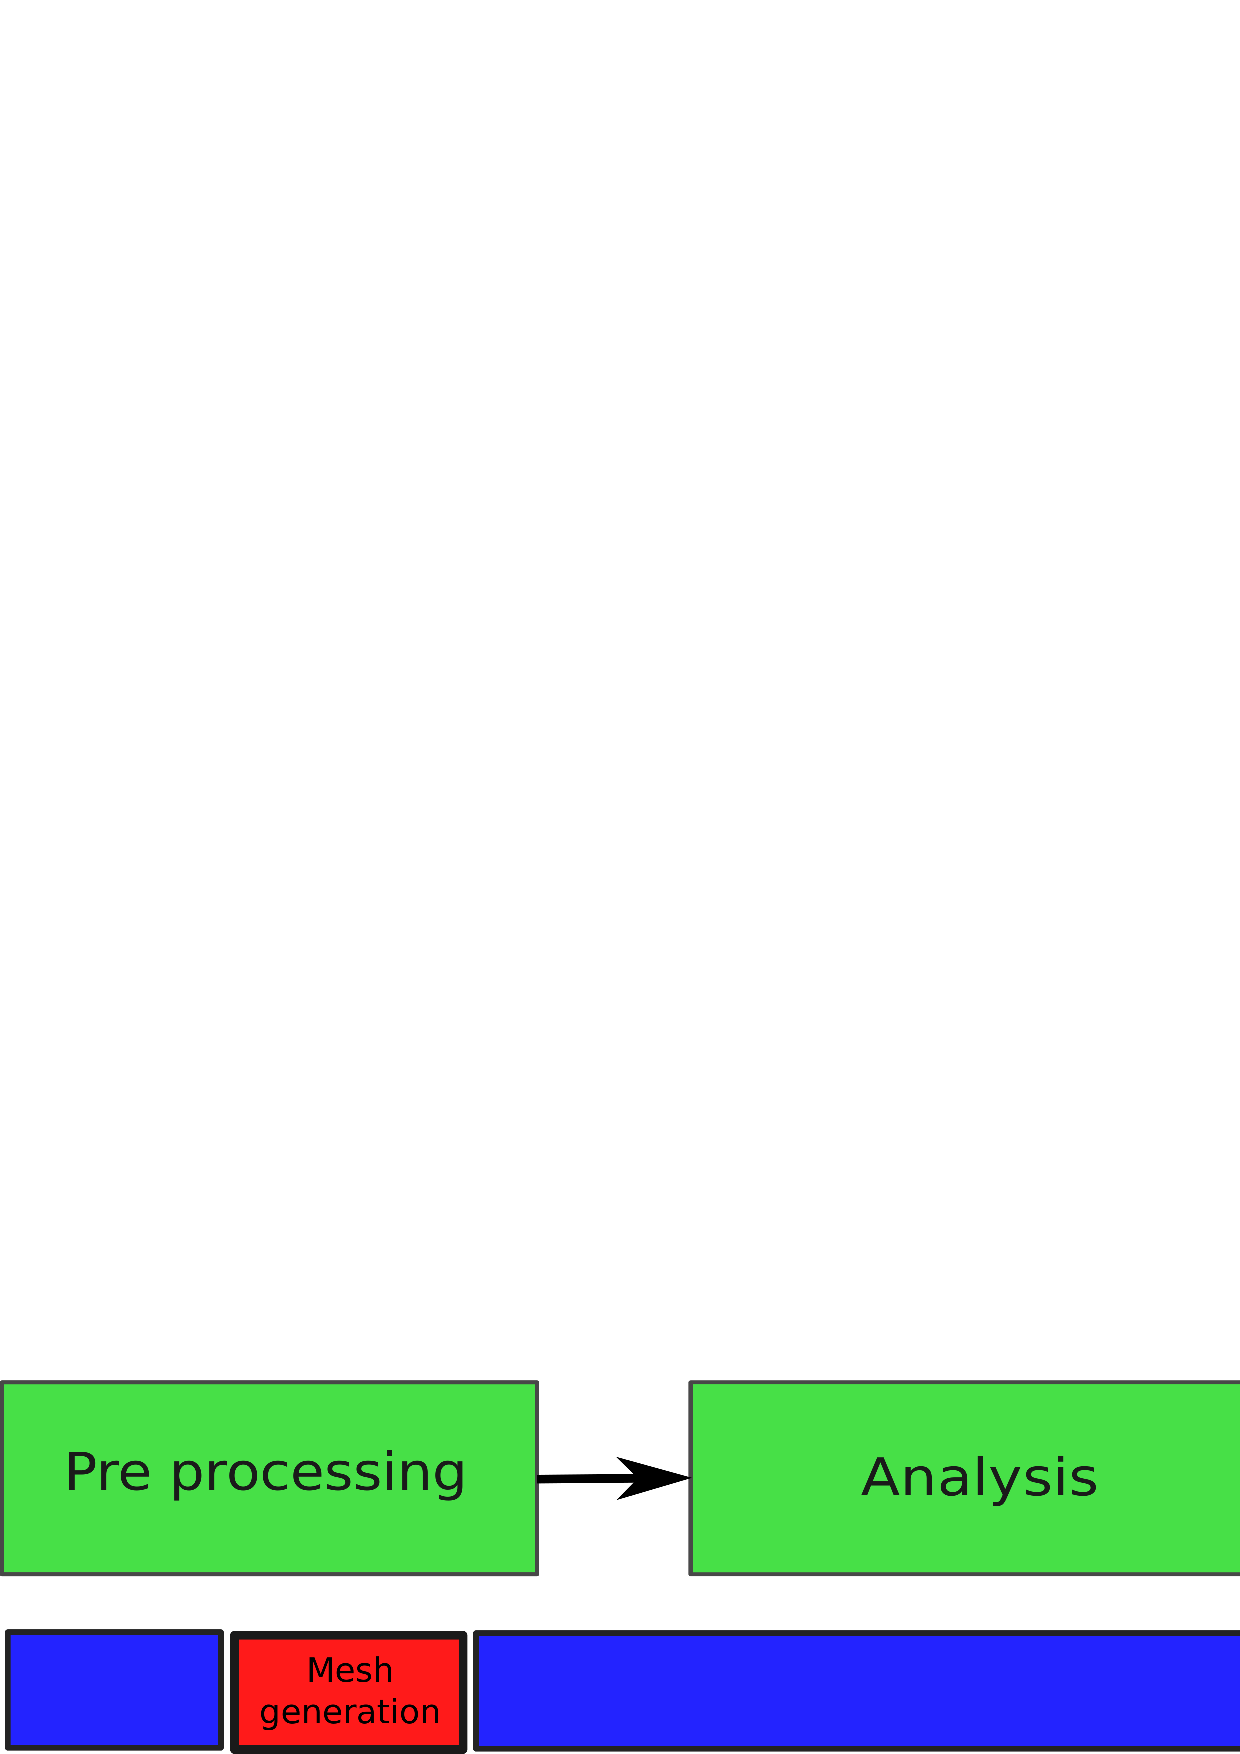
\includegraphics[scale=.3]{./img/stages_comparison.pdf}
\caption{Representation of how much of the simulation process is performed by using PeyeQM's routines.}
\label{fig:stages_comp}
\end{figure}  
%
The following is a brief description of what is done in each stage:

\subsection{Pre-Processing}
Pre-Processing is the stage where we describe the problem that will be solved, in terms that are readily interpreted by the analysis (processing) stage. In other words, is what we need to do before solving. Comparing simulating to cooking this would be the moment when we choose and chop the ingredients as well as heating the stove. Preparing the ingredients in FEM means to:
\begin{itemize}
\item Define the geometry or domain of the simulation, with its regions and associated materials.
\item Define what kind of physics rule the problem, and what kind of solution we want.
\item Discretize or divide the domain in nodes and elements by using a meshing algorithm. 
\item Set boundary and initial conditions.
\item Based on the physics of the problem, build a system of equations that relate all of the above.
\end{itemize} 
 
\subsection{Analysis}
In the Processing or Analysis stage, we take the system of equations that has been constructed in the first stage and solve it using the respective numerical methods. If we have a stationary problem then  we have to solve a system of linear equations, if it is an eigenvalue problem, then we have find the eigenvalues and vectors of a certain matrix, and if it is an explicit solution then we must loop over unknowns assigning values. All in all, what we will do in this stage is the equivalent to the actual cooking of the ingredients. 

\subsection{Post-Processing}
Post processing, is to get the solution produced by the solver and serve it in a portioned and digestible way. In this step we will generally produce graphs, plots, and animations that represent the characteristic of the simulated phenomenon. If Pre-Processing was a sort of codification from human language to algorithm, then Post-Processing is a way of de-codification, from numbers to ``human''.

\section{Classes, Diagrams and flow charts of PeyeQM}
PeyeQM follows this basic Scheme but divides the Pre-Processing stage in two, one part is the assembling of the simulation and the second is the codification or interpretation of that simulation. Figure \ref{fig:stages_2} shows the interpretation that we have made of the  steps to follow.
\begin{figure}[h]
\centering
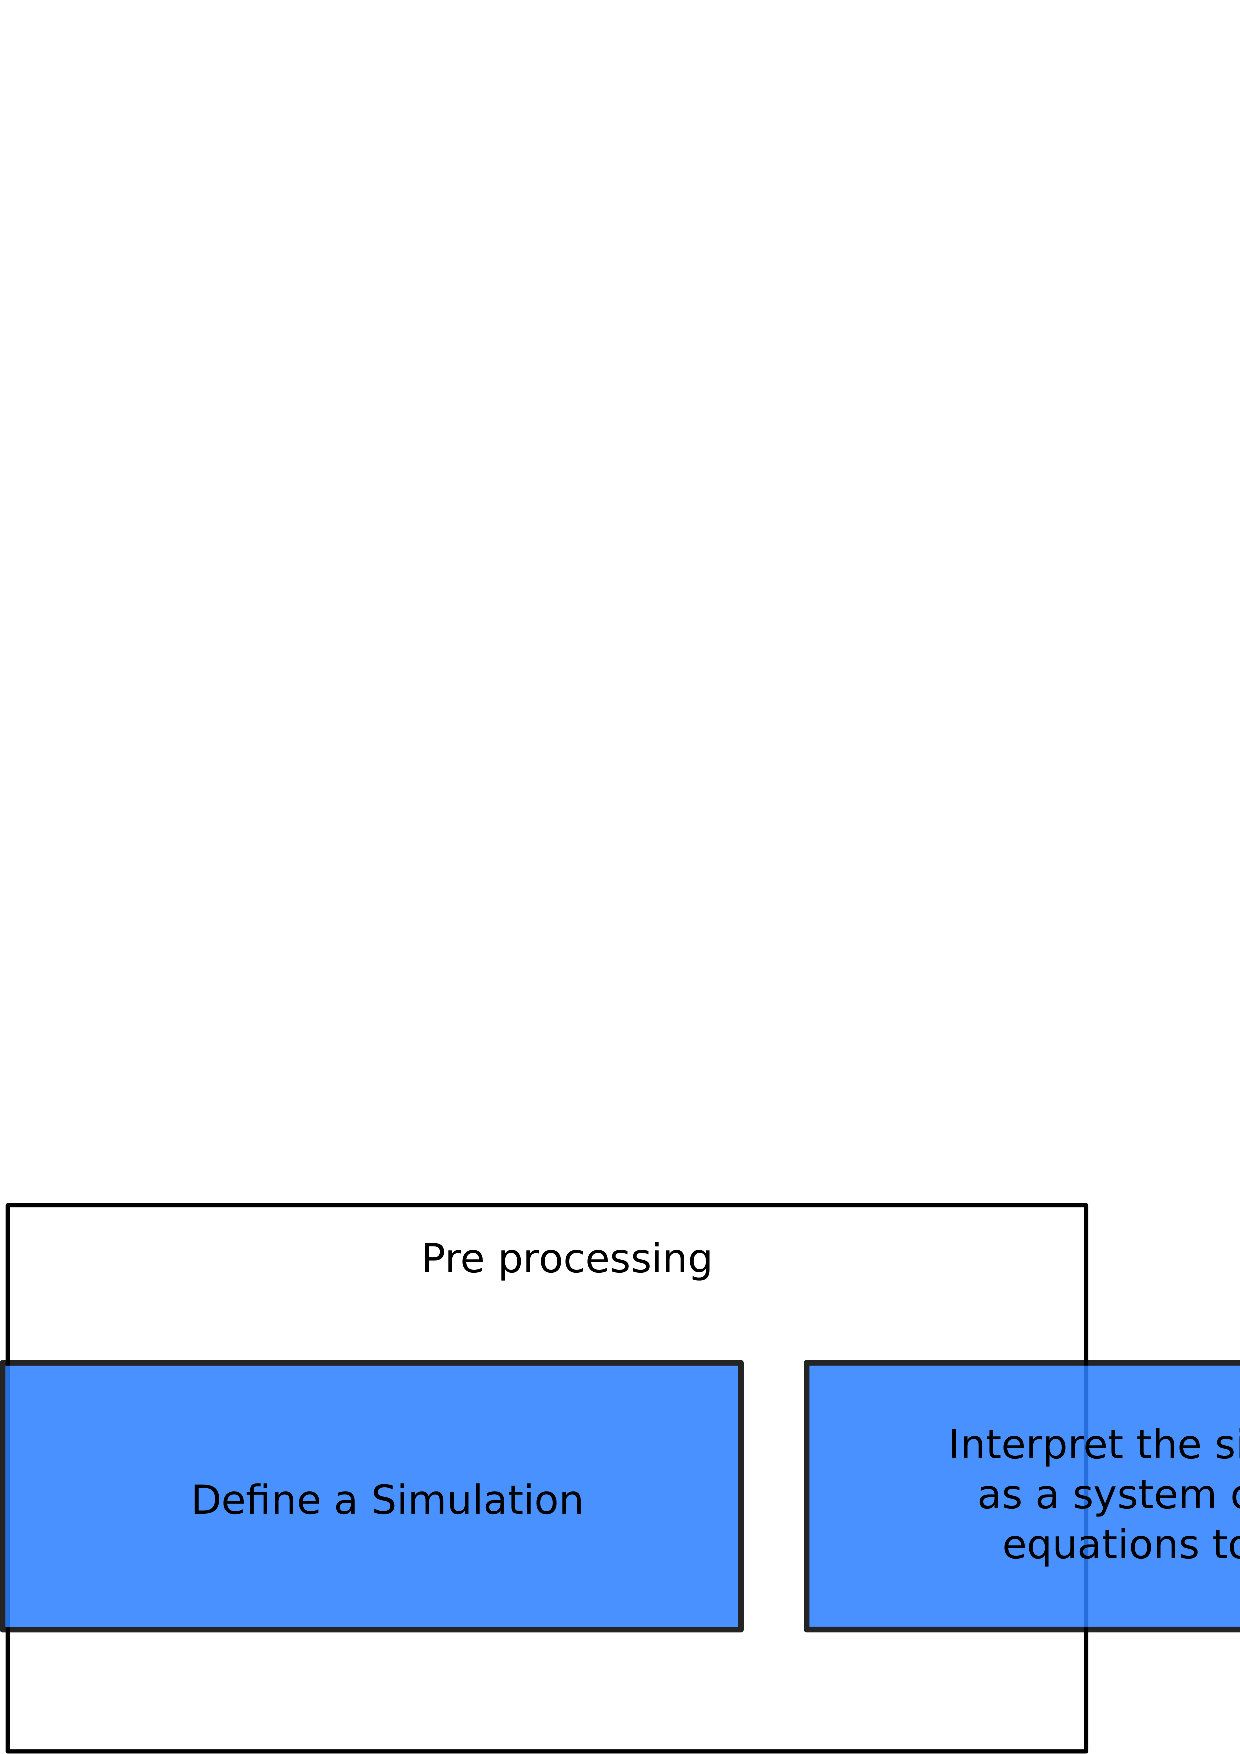
\includegraphics[scale=0.3]{./img/stages_abstract.pdf}
\caption{Diagram of general simulation stages as abstracted by PeyeQM.}
\label{fig:stages_2}
\end{figure}

The way in which we formulated the program in the context of OOP was to use three main classes that deal with the flow of chart \ref{fig:stages_2}.
\begin{itemize}
\item A \textit{Simulation} class,
\item \textit{Interpreter} class, and
\item \textit{Solver} class.
\end{itemize}
In that way, a simulation can interpreted as a kind of conversation between the user and members (instances or objects) of those classes. The first part of that conversation would be the user telling what he wants to a member of class \textit{Simulation}. Doing so the object ``simulation'' gets informed of the parameters needed to solve the problem.  The solver however does not understand either human language or the simulation language, and it needs some intermediary to hear what the simulation has to say and translate it as systems of equations which are its language. This new character is called the Interpreter and is a member of class \textit{Interpreter}. The interpreter is capable of reading the simulation and depending on the kind of physical problem, conditions and domain, will build the matrices and vectors mentioned in chapter \ref{ch:Finite_element_method}, and assemble them in the form of an equation. At this point of the conversation, the Solver, who is a member of class \textit{Solver} will listen to the interpreter and proceed to diligently solve the problem. Whenever the solution is ready it will then return the solution as a file that is in a predefined format, this file will then be passed to the Post-Processor, who will paint the solution for the user closing the loop of this conversation\footnote{It is important to remember now that we are using an external tool called Paraview for the visualization of data.}. 

A diagram showing the main classes that form a Simulation in PeyeQM can be seen in figure \ref{fig:classes}.

\begin{figure}
\centering
\includegraphics[scale=0.35]{./img/class_diagram.pdf}
\caption{This diagram shows the main classes defined PeyeQM. Classes that are called by a method are connected with lines that end with a black diamonds, and classes that are attributes of other classes are connected by white diamonds.}
\label{fig:classes}
\end{figure}

\section{PeyeQM usage}
The best way to explain how to use the platform is with an example. As it is right now, the platform works by using Python scripts\footnote{Programs that can interpret and automate the execution of tasks which could alternatively be executed one-by-one by a human operator.} that can be run by a computer that has Python console installed. In this section we will explain each line of a script  file (called \href{https://github.com/bebopsan/peyeQM/blob/Depuration/Lib/OOPyQM/Examples/Square\%20waveguide/Waveguide.py}{Waveguide.py}) used to simulate the field inside a wave guide\footnote{A proper explanation of what is a waveguide is made in chapter \ref{ch:Results}}, hoping that with that the reader gets an idea of how to use the libraries and encouraging him-her to explore the examples that have been uploaded in the repository. 

Starting from the first two lines we define what to use in order to execute the file and the kind of coding:
\begin{python}[language=python]
#!/usr/bin/python
# -*- coding: utf-8 -*-
\end{python}

The next part is the doc string of the script, this is what appears if from inside python you type \verb|help(Waveguide.py)|. The documentation will include the file types that are needed and will also give a brief summary of what the file does.

\begin{python}[language=python]
"""
Created on Sat Apr  6 18:58:29 2013

This script solves the harmonic wave equation for electromagnetic fields in 
a rectangular waveguide.

It reads the files with name stated in variable filename.

The necessary files are files with following extensions:
    
    .msh    Mesh file has information about nodes and elements
    .reg    Information about regions and material properties
    .bc     Boundary conditions pertinent for the simulation

The output will be a set of .vtk files written with the same name of write_solver_input.
The number of results depends on the number of eigenvalues and eigenvectors you wish
to compute.

Pseudo:
------
 - Define path of main libraries
 - Import classes and functions 
 - Define filename of input files
 - Define all the initial conditions that make the simulation and save them 
    into the mesh file.
- Instantiate and populate the simulation
    - add a domain by reading from the mesh
    - add boundary conditions from .bc
    - add regions definitions from .reg
- Instantiate  the Interpreter and build the equation for harmonic problem
- Instantiate the solver and solve the equation for spectral problem
- fit the solution for a three component array, and export it to vtk files

@author: Santiago Echeverri Chacon
"""
\end{python}

Following that, (and as mentioned in the docstring) we have the definition 
of absolute path for the libraries that contain classes and functions, this is needed if the script is in a folder and not in the root directory of the libraries:
\begin{python}
import os, sys
lib_path = os.path.abspath('../..')
sys.path.append(lib_path)
\end{python}
And then, we import the classes in order to use them afterwards:
\begin{python}
from Classes import Simulation
from Interpreter import Interpreter
from Solver import Solver
from write import write_vtk, write_solver_input 
from numpy import zeros
\end{python}

For convenience all the input files share the same name. We define the name and also write in the \verb|.msh| file the conditions of the simulation. In the second statement we are saying that this will be a 2D Electromagnetic problem with Dirichlet conditions, and that it can find for boundaries if it looks in file with name filename and extension \verb|.bc|:
\begin{python}
filename = 'square_waveguide'
write_solver_input(filename +'.msh',dimension = 2, bc_type = 'Dir', \
parameter = [], eq = 'EM', sol_type = 'Stationary',analysis_param \
= ['y', 'y', 15, 15, 20, 20, 2], bc_filename = filename +'.bc')  
\end{python}

Afterwards, we initialize an instance of class simulation and read the  information that was written in the mesh  with the method \verb|read_solver_input()|. The nodes and elements are assigned to subclass Domain, by using the function \verb|read_mesh_file()|. Boundary conditions are assigned to the domain by invoking the method \verb|read_bc_file()|, and regions of the domain are defined by reading the \verb|.reg| input file with method \verb|read_regions_file()|.

\begin{python}
simu = Simulation()
simu.read_solver_input(filename +'.msh')
simu.domain.read_mesh_file(filename +'.msh', True)
simu.domain.read_bc_file(simu.bc_filename)
reg_filename = simu.bc_filename.split('.bc')[0]
simu.domain.read_regions_file(reg_filename)
\end{python}

At this point the simulation is fully defined and ready to be interpreted. So, in the next lines we instantiate the interpreter and call the routine that builds the equation for harmonic fields. Notice that the argument of the function that assembles the equation is the instance of the simulation, so the interpreter has full access to everything we defined before.

\begin{python}
inter = Interpreter()
eq = inter.build_harmonic_EM_eq(simu)
\end{python}

The next step is to call the solver and solve with the routine for harmonic simulations \verb|solve_spectral()|. The output of the solver is an array with the eigenvalues and another array with the respective eigen functions.

\begin{python}
my_solver = Solver()
value, fields = my_solver.solve_spectral(simu, eq)
print len(fields), 'value', value
\end{python}

After this command the eigenvalues are printed in the console. The following code snippet is not very well organized, but what it does is to lower the numbering of the elements by one because \verb|.vtk| files use numbering that starts in 0. After that we format the fields that have two components into an array in which the third component $z$ is assumed to be zero for every node. This is because \verb|.vtk| requires that all components of a vector field are defined.

\begin{python}
quads = my_solver.substract_1(simu.domain.elements.quads.el_set)
quads = quads[:,1:]
for i in range(len(fields)):
    field3 =  zeros((simu.domain.nodes.n,3))
    field3[:,0:2] = fields[i]
    fields[i] = field3
\end{python}

The final line of code is for writing into \verb|.vtk|  format. We use function \verb|write_vtk()| and give it the nodes, elements and vector fields as arguments.
\begin{python}
	write_vtk(filename +str(i)+'.vtk', 'MyTitle', 'UNSTRUCTURED_GRID' \
	 ,simu.domain.nodes.coords,\	 				
        quads, ['VECTORS', ['sol'], [fields[i]]])
\end{python}

\section{Python}
The software platform developed as part of this project was entirely written in \href{http://www.python.org/Python}{Pyhon}. Numerical routines for handling of matrices and the solution of systems of equations, or eigenvalue problems where taken from python based  scientific packages: \href{http://www.scipy.org/}{scipy} and \href{http://www.numpy.org/}{numpy}

Python is a \href{http://en.wikipedia.org/wiki/High-level_programming_language}{high level programing language} oriented towards \href{http://en.wikipedia.org/wiki/Dynamic_programming_language}{dynamic objects}. Moreover it has been designed such that it  emphasizes code readability, Python's syntax allows programmers to express concepts in fewer lines of code than would be possible in low-mid level compiled languages such as C. It is thus similar to Matlab and JavaScript in the sense that it is an interpreted programming language that does not need compiling, and is supported in multiple platforms. Being so, it sacrifices some performance with optimization of developing time in  mind\cite{Georgatos2002}. 
Python is often used as a scripting language, it can call and execute other programs and it allows wrapping of routines written in low level languages like C. All of these properties make it a relevant tool for teachers, scientists and engineers whose priority is development speed and clarity over machine level high performance \cite{Villegas2011, Kiusalaas2005, Baecker2007, Euroscipy2010, Borcherds2007, Langtangen2004}.

\section{Gmsh}
\begin{quote}
``Gmsh is a 3D finite element grid generator with a build-in CAD engine and post-processor. Its design goal is to provide a fast, light and user-friendly meshing tool with parametric input and advanced visualization capabilities'' \cite{Geuzaine2009}. 
\end{quote}
We used Gmsh as both a Computer Aided Design (CAD) tool and mesh generator for the modelling of simulation domains used in most part of the results presented in \ref{ch:Results}. It could be said that Gmsh is the main pre-processing tool used by PeyeQM.

Gmsh CAD and meshing modules are design such that its input and output can be parsed using ASCII text files written in Gmsh's own scripting language. In this project we took advantage of this, and developed the input format of the simulator over the same syntax as Gmsh otuput \verb|.msh| mesh files. Moreover, PeyeQM's module for the creation of geometries (\verb|gmsh_library.py|) used to define finite crystals with defects, exports geometry files \verb|.geo| that   are proper inputs for Gmsh. Using that module we can bypass the CAD module of Gmsh and construct arbitrary crystal-like geometries that are be interpreted and meshed by the meshing tool of Gmsh. The main classes used to define geometrical objects that are then translated to gmsh syntax are shown in the diagram of figure \ref{fig:gmsh_library_classes}


\begin{figure}
\centering
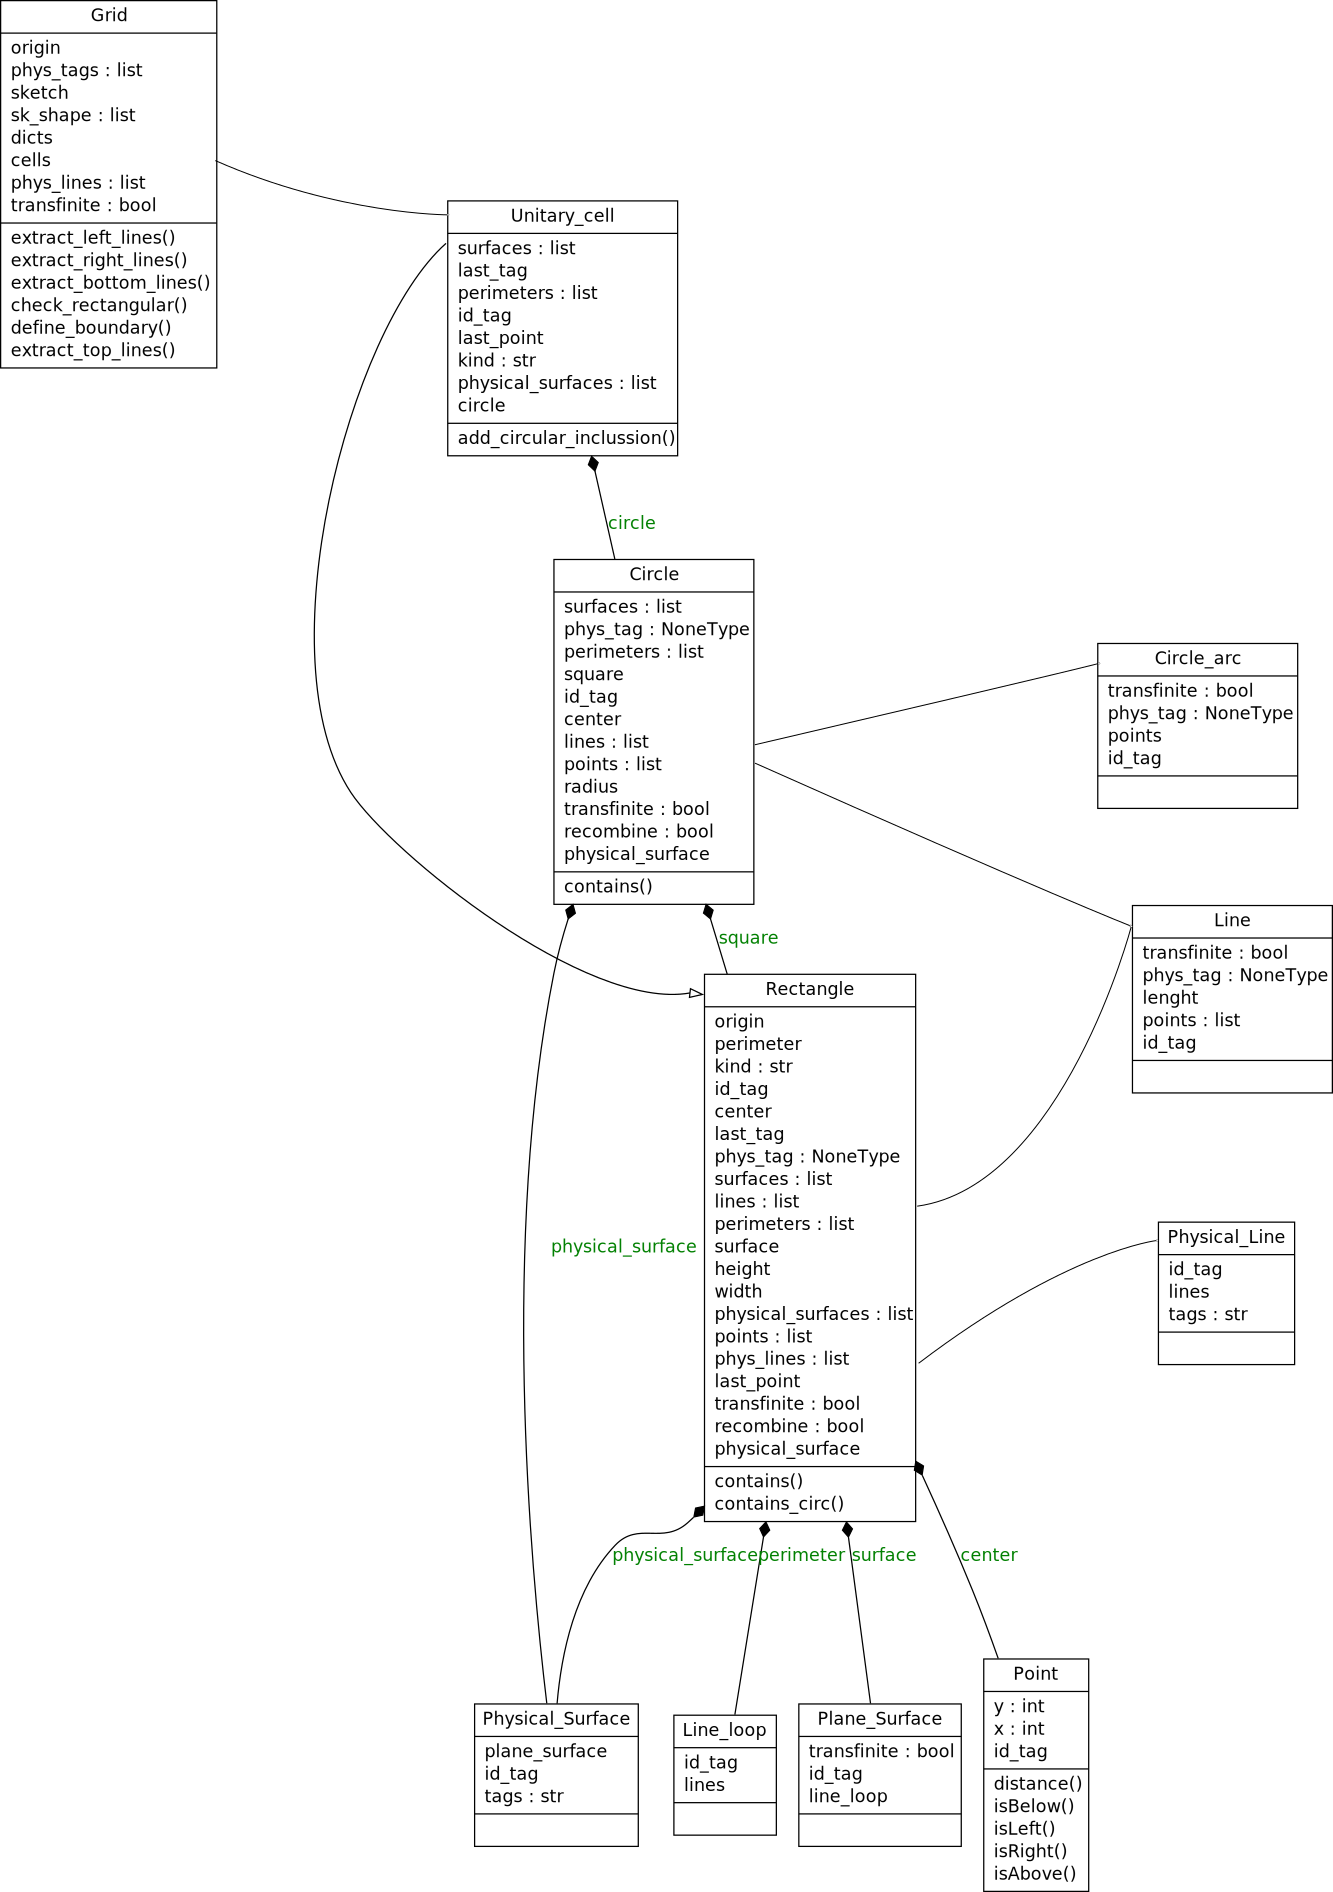
\includegraphics[scale=0.33]{./img/gmsh_library.pdf}
\caption{This diagram shows the classes defined in the module gmsh\_library.py. Classes that are called by a method are connected with lines that end with a black diamonds, inheritance is shown with a white arrow, and classes that are attributes of other classes are connected by white diamonds.}
\label{fig:gmsh_library_classes}
\end{figure}

\section{Paraview}
\begin{quote}``ParaView is an open-source, multi-platform application designed to visualize data sets of size varying from small to very large'' \cite{Henderson2007, ParaviewDoc}.\end{quote}
It is built on top of the Visualization Tool Kit libraries(VTK), so given a \textit{.vtk} file format that contains data one can generate all sorts of graphs and plots from it, and interactively extract quantitative and qualitative information. 
Paraview is used externally in this implementation as the principal post processing tool. The  solution of FE simulations is saved to \textit{.vtk} files by means of writing with routine \verb|write_vtk()| found in library \href{https://github.com/bebopsan/peyeQM/blob/Depuration/Lib/OOPyQM/write.py}{write.py}. All the images from chapter \ref{ch:Results} (except for dispersion plots) were generated using Paraview.




\chapter{Results}
\label{ch:Results}
As mentioned in the introduction, a software platform able to simulate propagation of electromagnetic waves in photonic crystals was developed. In chapter \ref{ch:Electromagnetic waves in periodic media} the equations that rule the problem where stated, and background behind one method of solution for them using FEA has been discussed in chapter \ref{ch:Finite_element_method}. In this chapter the solutions obtained by applying these concepts are presented and compared with either their analytic solutions or numerical solutions from the literature.

\section{Electrostatic benchmark tests}

Now, platform \href{https://github.com/bebopsan/peyeQM}{PeyeQM} was built in a \href{en.wikipedia.org/wiki/Top-down_and_bottom-up_design}{bottom-up } process that started by making a FE solver that could handle static scalar problems of electron confinement in 2D potential wells for application in Quantum Mechanics. This project involved an upgrade of that platform that began with the implementation of support for vector formulations, and a transition to Object Oriented Paradigm that could improve flexibility and maintenance.

The first section of this chapter shows the results obtained for Electrostatic benchmark tests, and were made in order to assert the accuracy of the static vectorial solver, and  routines for the construction of stiffness matrices.

\subsection{Electric field due to charged elements}
\subsubsection{Parallel plate capacitor}
The first experiment was to simulate the most basic field we could think of, this is, that inside a parallel plate capacitor, where field lines go straight from one plate to the other. 

Electric fields satisfy equation \ref{eq:diff_Faraday}. If there are no sources or sinks ($- \frac{\partial \mathbf{B}}{\partial t}=0)$, then the field $\mathbf{E}$ is said to be \textit{irrotational} and by an \href{http://ebooksgo.org/mathematics/Vector_Identity.pdf}{identity of vector} calculus we know that there must exist a scalar field $V$ whose gradient is a valid Electrostatic vector field:
\begin{equation}
\nabla\times\nabla V = 0
\label{eq:Laplace}
\end{equation}
Scalar equations are easier to solve and are very useful when the medium is homogeneous and isotropic, this is the reason why many books stick with scalar problems and leave the process of obtaining $\mathbf{E}$ as performing on $V$ the derivations in operator $\nabla$. Using the scalar potential as an intermediate step for the solution of $\mathbf{E}$ stops being a good idea when interfaces between mediums and sharp geometries appear, and a direct solution using vector fields gains relevance.

In a parallel plate capacitor like that in figure \ref{fig:parallel_plate}, we consider two (infinite, parallel, plane, perfectly conducting, charged) plates that occupy the planes $x = 0$ and $x = d$ kept at potentials $V = 0$ and $V = V_0$ respectively.  
With plates of very large dimensions compared to the spacing between them, the potential becomes a function of $x$ only, and equation \ref{eq:Laplace} becomes:
$$\dfrac{d^2V}{d x^2}=0$$ Integrating twice, we get: 
\begin{equation}
V(x) = Ax + B
\end{equation}
Where $A$  and $B$ are constants of integration solved by using boundary conditions.
$$V(0) = A0 + B = 0 \quad or \quad B = 0$$$$V(d) = Ad + B = V_0 \quad or \quad A = \dfrac{V_0}{d}$$

Making the particular solution for the potential:
$$V=\dfrac{V_0}{d}x \quad for \quad 0<x<d$$ 
The field is then obtained by taking the gradient of $V$, and we add a $-$ sign taking into account that $\mathbf{E}$ is a conservative field.

\begin{equation}
\mathbf{E}= -\nabla V = - \dfrac{dV}{dx}\hat{a}_x = -\dfrac{V}{d}\hat{a}_x
\end{equation}
 This means that the field is uniform and directed from the higher potential plate to the lower potential plate as shown in \ref{fig:parallel_plate} \ref{Rao2004}.

\begin{figure}
\centering
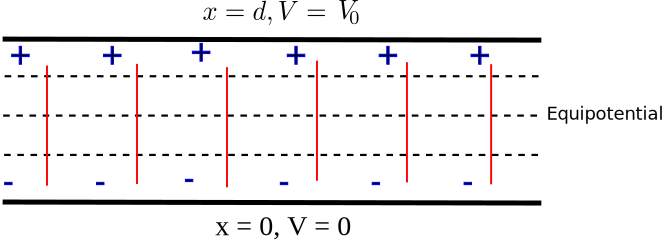
\includegraphics[scale=0.5]{./img/parallel_plate_capacitor.pdf}
\caption{Cross sectional view of parallel plate capacitor.}
\label{fig:parallel_plate}
\end{figure}

A rectangular region was meshed and Dirichlet boundary condition were applied in the bottom and top plates as a field pointing down. Separation $d$ is taken unitary and the result is shown in figure \ref{fig:capacitor}.

\begin{figure}
\centering
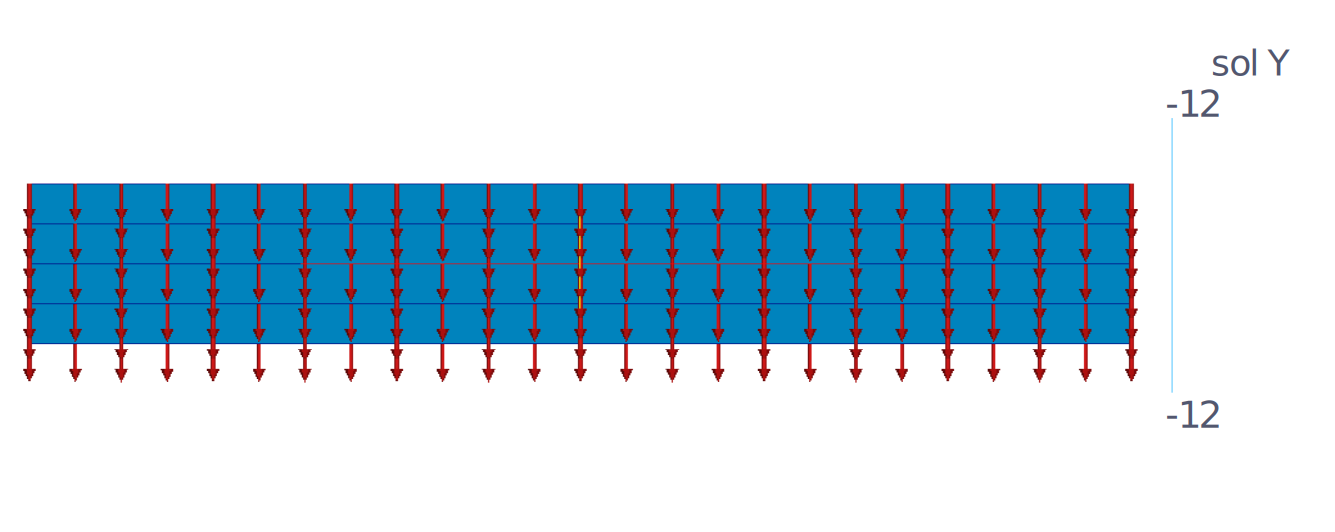
\includegraphics[scale=0.3]{./img/capacitor.pdf}
\caption{Solution of electric field in parallel plate capacitor.}
\label{fig:capacitor}
\end{figure}

It can be seen that the lines don't change in either magnitude or direction, and go from the charged plate wit potential $V_0$ to the bottom plate as expected.

This test showed that the routines for assembling stiffness matrices are capable of continuing a simple field over a distance between to boundaries.

The script for producing this simulation and the necessary input files can be seen in the 
\href{https://github.com/bebopsan/peyeQM/tree/Depuration/Lib/OOPyQM/Examples/Capacitor}{\textit{repository}.}

\subsubsection{Charged cylinder}

The next field problem to solve in order to test PeyeQM was one with circular geometry. The solution for the field due to a point charge or a charged cylinder was used to compare the precision of the method for representing fields with two components.

Gauss law \ref{eq:Gauss} in spherical coordinates, assuming a homogeneous medium with scalar permittivity is:

\begin{equation}
\epsilon \int_S \mathbf{E}\cdot d\mathbf{S} = \int_V \rho dV
\end{equation}

Where $\int_V \rho dV = q$ is the charge of the particle. If that charge is distributed uniformly, then there are no preferred directions and the electric field must be radial \cite{Cheng1993} and have constant intensity over spherical shells. So for an arbitrary 
spherical shell of radius $r$:

\begin{align*}
&\epsilon \mathbf{E} \int_{\theta}\int_{\phi} r^2 sin(\theta) d \phi = q \\
& \mathbf{E}_r(r) = \frac{q}{4\pi \epsilon r^2} \hat{r}
\end{align*}
Now, this has to be transformed into Cartesian coordinates in order to input boundary conditions. If we consider $r$ as the magnitude of vector $\vec{r}$ in the unitary direction $\hat{r}$ then we can transform it to a linear combination of unitary vectors $\hat{x}$ and $\hat{y}$ by the following:
\begin{equation}
\vec{r} = r cos(\theta) \hat{x} + r sin(\theta) \hat{y}
\end{equation}
And by trigonometry we know that $cos(\theta) =\dfrac{x}{r}$ and $sin(\theta)=\dfrac{y}{r}$. Making the necessary substitutions we get to:

\begin{equation}
\mathbf{E}_r(r) = \mathbf{E}_x(x,y) + \mathbf{E}_y(x,y) = \frac{qx}{4\pi \epsilon \sqrt{\left(x^2+y^2\right)}^3} \hat{x}+\frac{qy}{4\pi \epsilon \sqrt{\left(x^2+y^2\right)}^3} \hat{y}
\end{equation}
So, a plot the solution after simulating should match a representation of this analytic result. We initially proposed a model where the charged cylinder or point source is modeled as a \href{https://github.com/bebopsan/peyeQM/tree/
Depuration/Lib/OOPyQM/Examples/Whole\%20cylinder}{whole circle inside a square domain}, the results of the simulation ( figure \ref{fig:whole_cylinder}) showed that for this kind of problem where the field decays in the form $\dfrac{1}{r^2}$ it was better to use finer meshes and take advantage of symmetries to reduce the computational cost. 
Taking just an eight of the model, and reshaping the outer boundary to a circle improved the quality of the elements and allowed us to use a finer mesh. figure \ref{fig:eight_of_cylinder} shows the $y$ and $x$ components of the field as well as the error between the simulation and the analytic solution.
For the simulation factor $\dfrac{q}{2\pi \epsilon}$ has been normalized to 1, and the mesh was done done using 1996 QUAD8 elements with 5525 nodes, thus 11050 degrees of freedom. As a comparison, the simulation of the whole circle involved 2432 elements and 7040 nodes with 14080 degrees of freedom, but it solved for a domain that was eight times bigger.


\begin{figure}
\centering
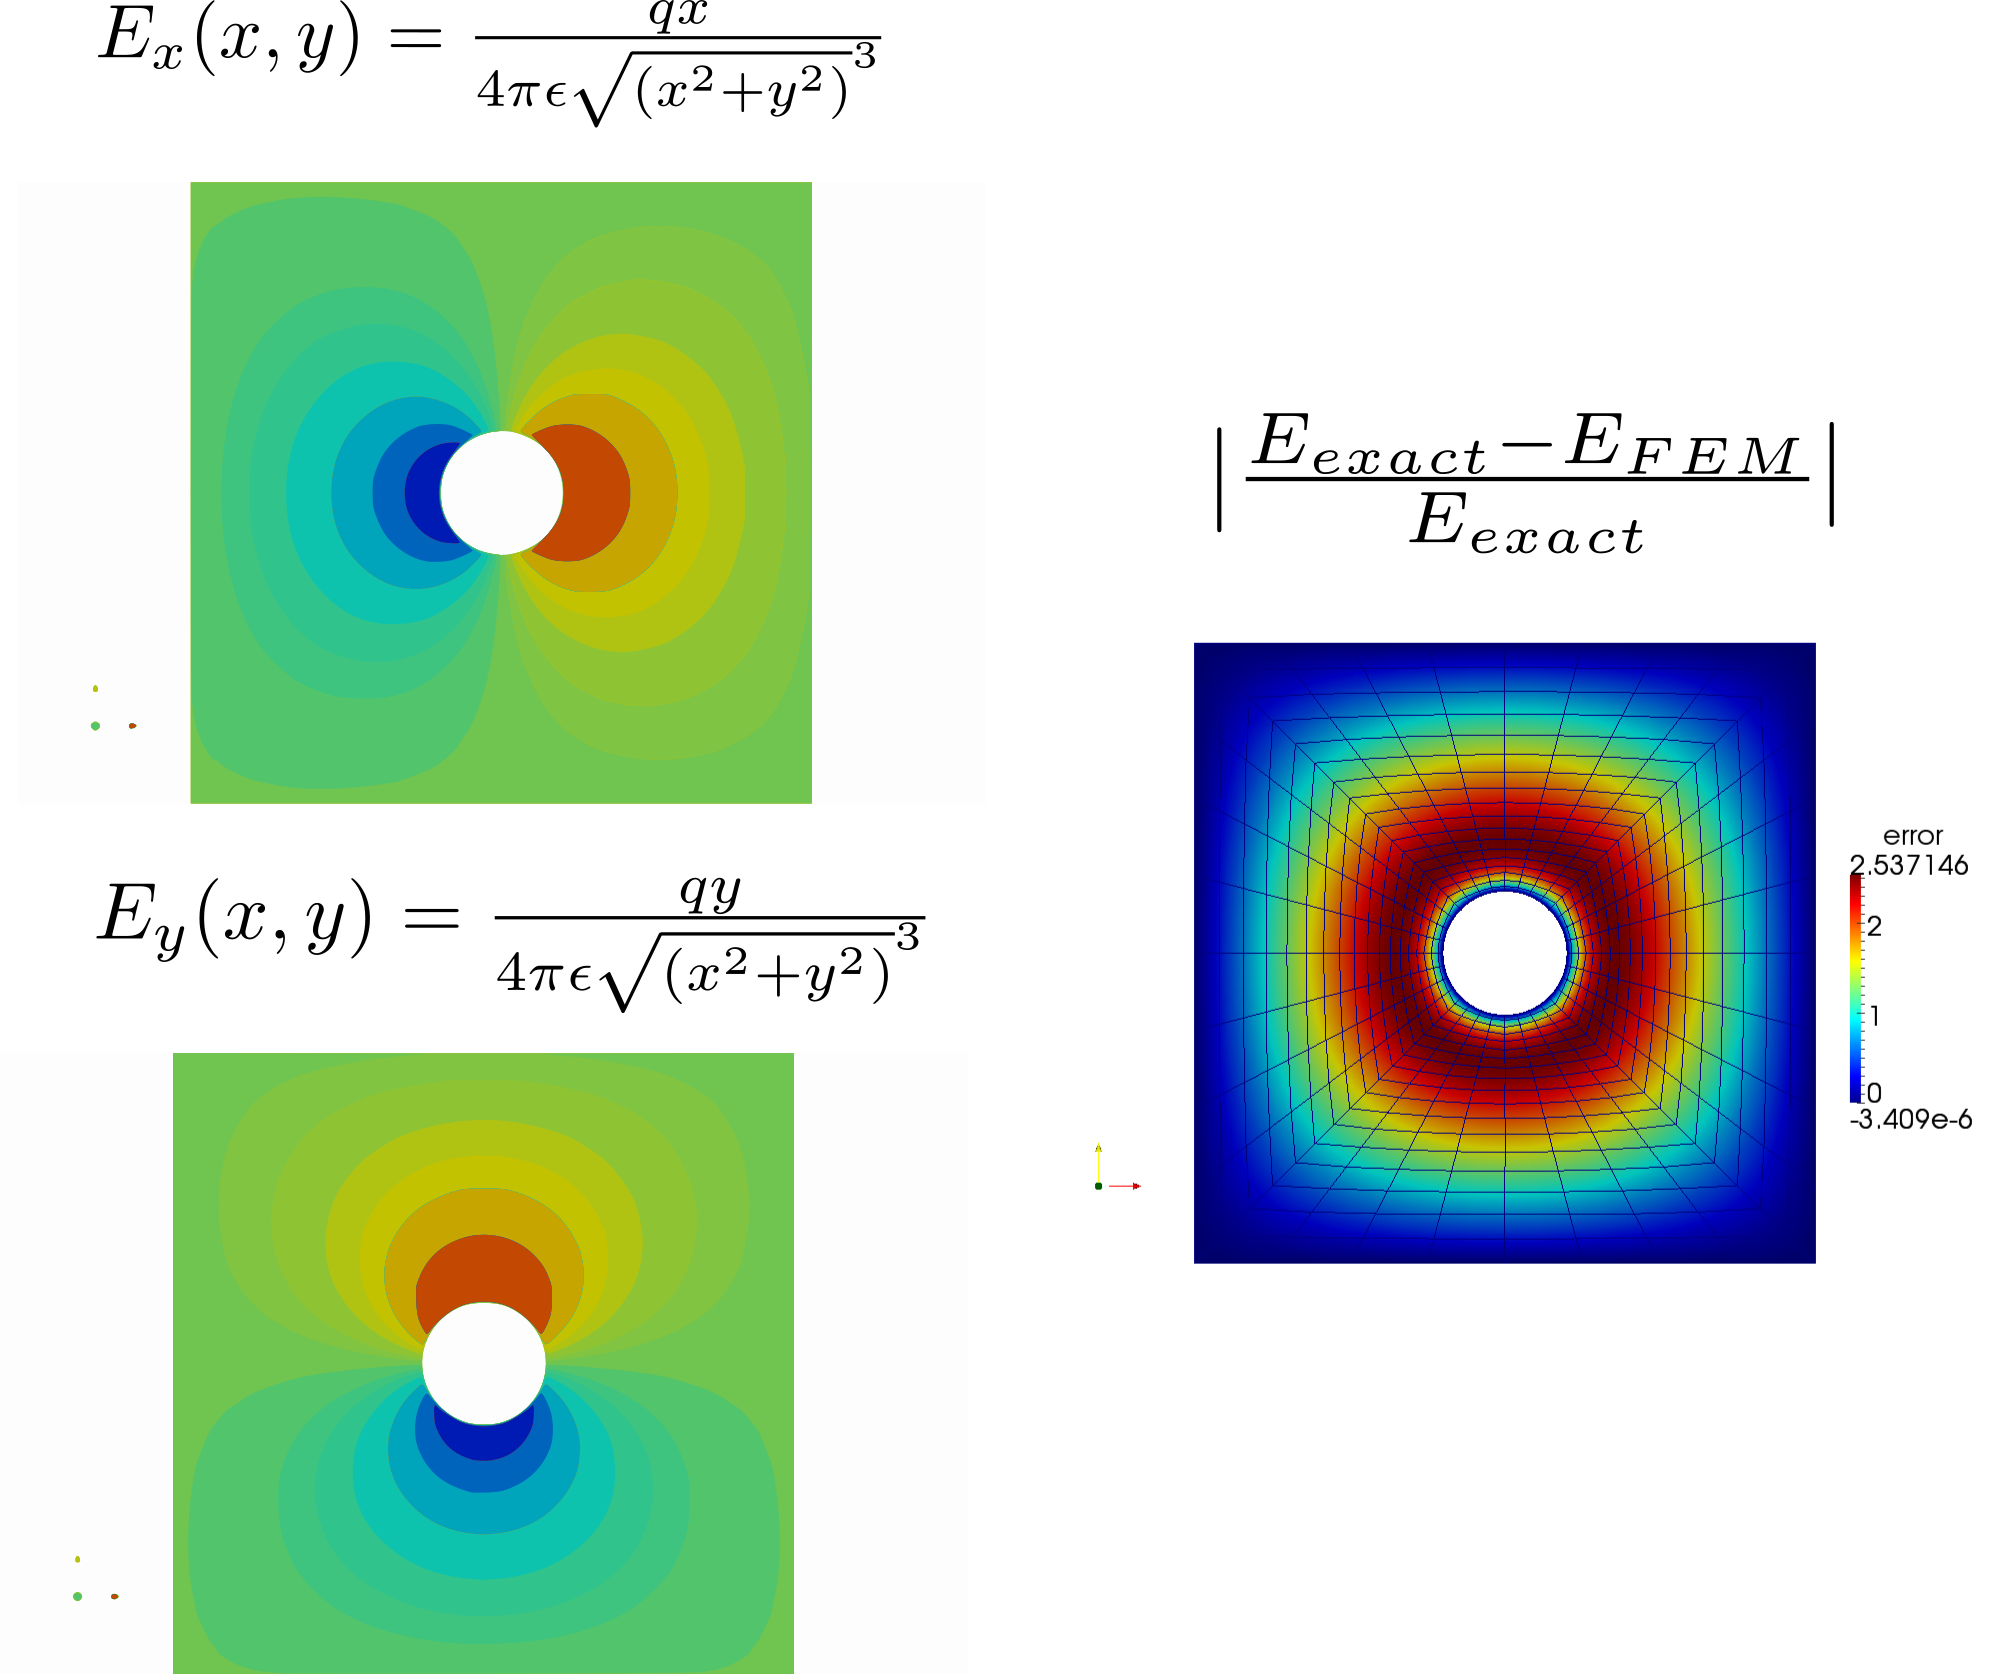
\includegraphics[scale=0.2]{./img/charged_cylinder_inside_rectangle.pdf}
\caption{Whole simulation of Electric field due to a charged cylinder. Left, Numerical result for the $x$ component of the field. Middle, $x$ component of the solution, and, right, mesh and error calculated between analytic formula and results.}
\label{fig:whole_cylinder}
\end{figure}
 
\begin{figure}
\centering
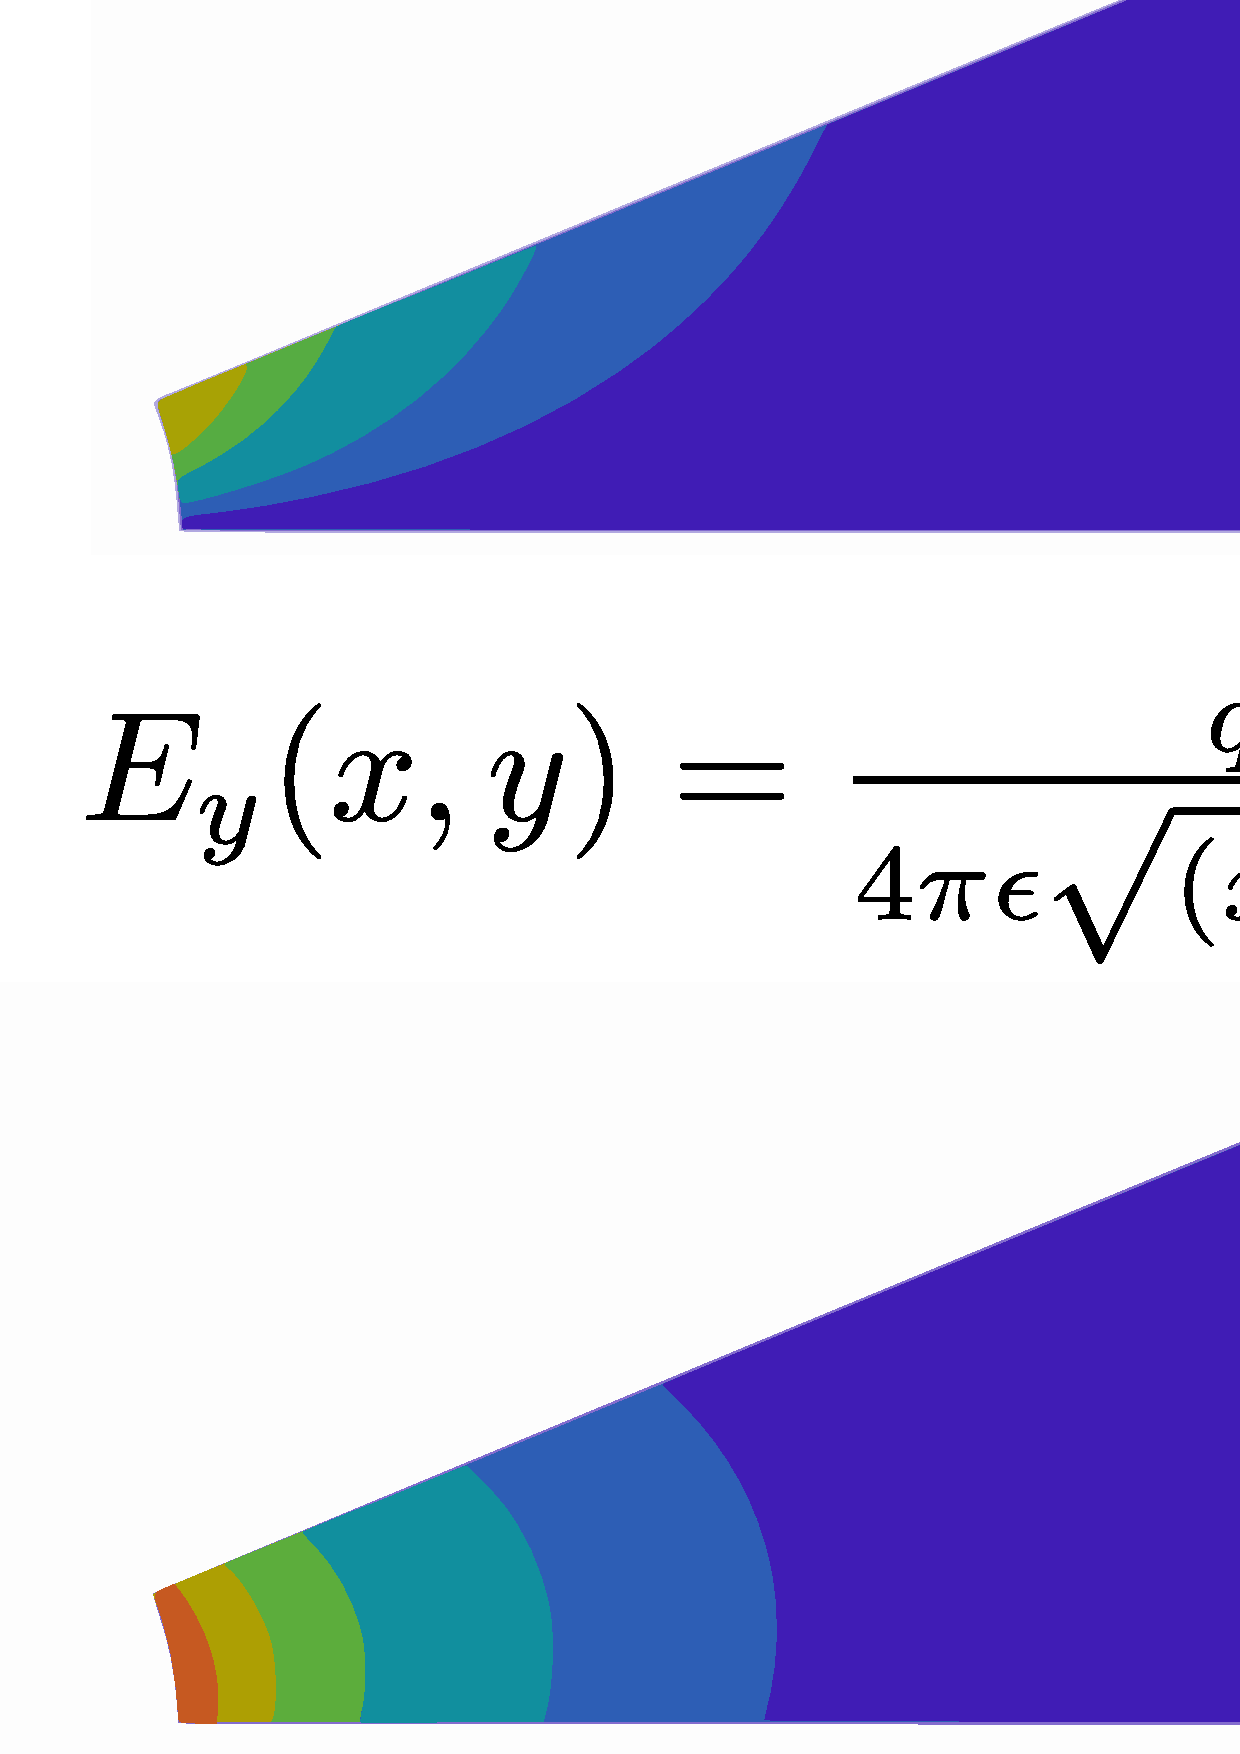
\includegraphics[scale=0.2]{./img/Eight_of_cylinder.pdf}
\caption{Segment of the simulation for Electric field due to a charged cylinder. a) Numerical result for the $y$ component of the field, b) x component of the solution, c) Mesh and error calculated between analytic formula and results.}
\label{fig:eight_of_cylinder}
\end{figure}

\subsubsection{Electric Dipole, two charged spheres.}

A similar simulation was performed using two semicircular surfaces, taking advantage of inversion symmetry along $x$ axis. Boundary conditions are Dirichlet conditions over the circles and the rectangular boundaries on top, and Neumann conditions set to 0 on bottom lines.  The analytic solution is simply the overlapping of the field due to charge 1 and charge 2, having one of them centered in the origin, and the other displaced by a distance $d$. The field everywhere can be expressed as: 

\begin{align}
&\mathbf{E}_1(x,y)=x\left(x^2+y^2\right)^{-\frac{3}{2}}\hat{x} + y\left(x^2+y^2\right)^{\frac{3}{2}}\hat{y}\\ 
&\mathbf{E}_2(x,y)=-(x-4)\left((x-4)^2+y^2\right)^{-\frac{3}{2}} \hat{x}-y\left((x-4)^2+y^2\right)^{\frac{3}{2}}\hat{y}\\
&\mathbf{E}_x = \left[ x\left(x^2+y^2\right)^{-\frac{3}{2}} -(x-4)\left((x-4)^2+y^2\right)^{-\frac{3}{2}}\right] \hat{x}\\
&\mathbf{E}_y =\left[ y\left(x^2+y^2\right)^{\frac{3}{2}} -y\left((x-4)^2+y^2\right)^{\frac{3}{2}}\right]\hat{y}
\end{align}

Where again $\dfrac{q}{2\pi \epsilon} = 1$ for the left charged circle and $-1$ for the one on the right at a distance $d=4$. Figure \ref{fig:two_cylinders} shows components $x$ and $y$ of the resulting field as obtained from the FE solver. The direction of the field lines can be observed by means of arrow glyphs in figure \ref{fig:two_cylinders_glyph}, where field lines go outwards in the positively charged cylinder and inwards in the negative.
In the same way as before, a comparison between analytic and numerical solutions was performed (figure \ref{fig:two_cylinders_error}) and error appeared to be magnified in the region between cylinders. This value keeps being higher than expected, and different meshing schemes were tested in order to improve accuracy. Less error was observed using adaptative meshing methods than structured grids. The current mesh for this simulation has 510 elements and 1622 degrees of freedom, a future simulation is proposed with finer meshes using a PC with bigger RAM.

\begin{figure}
\centering
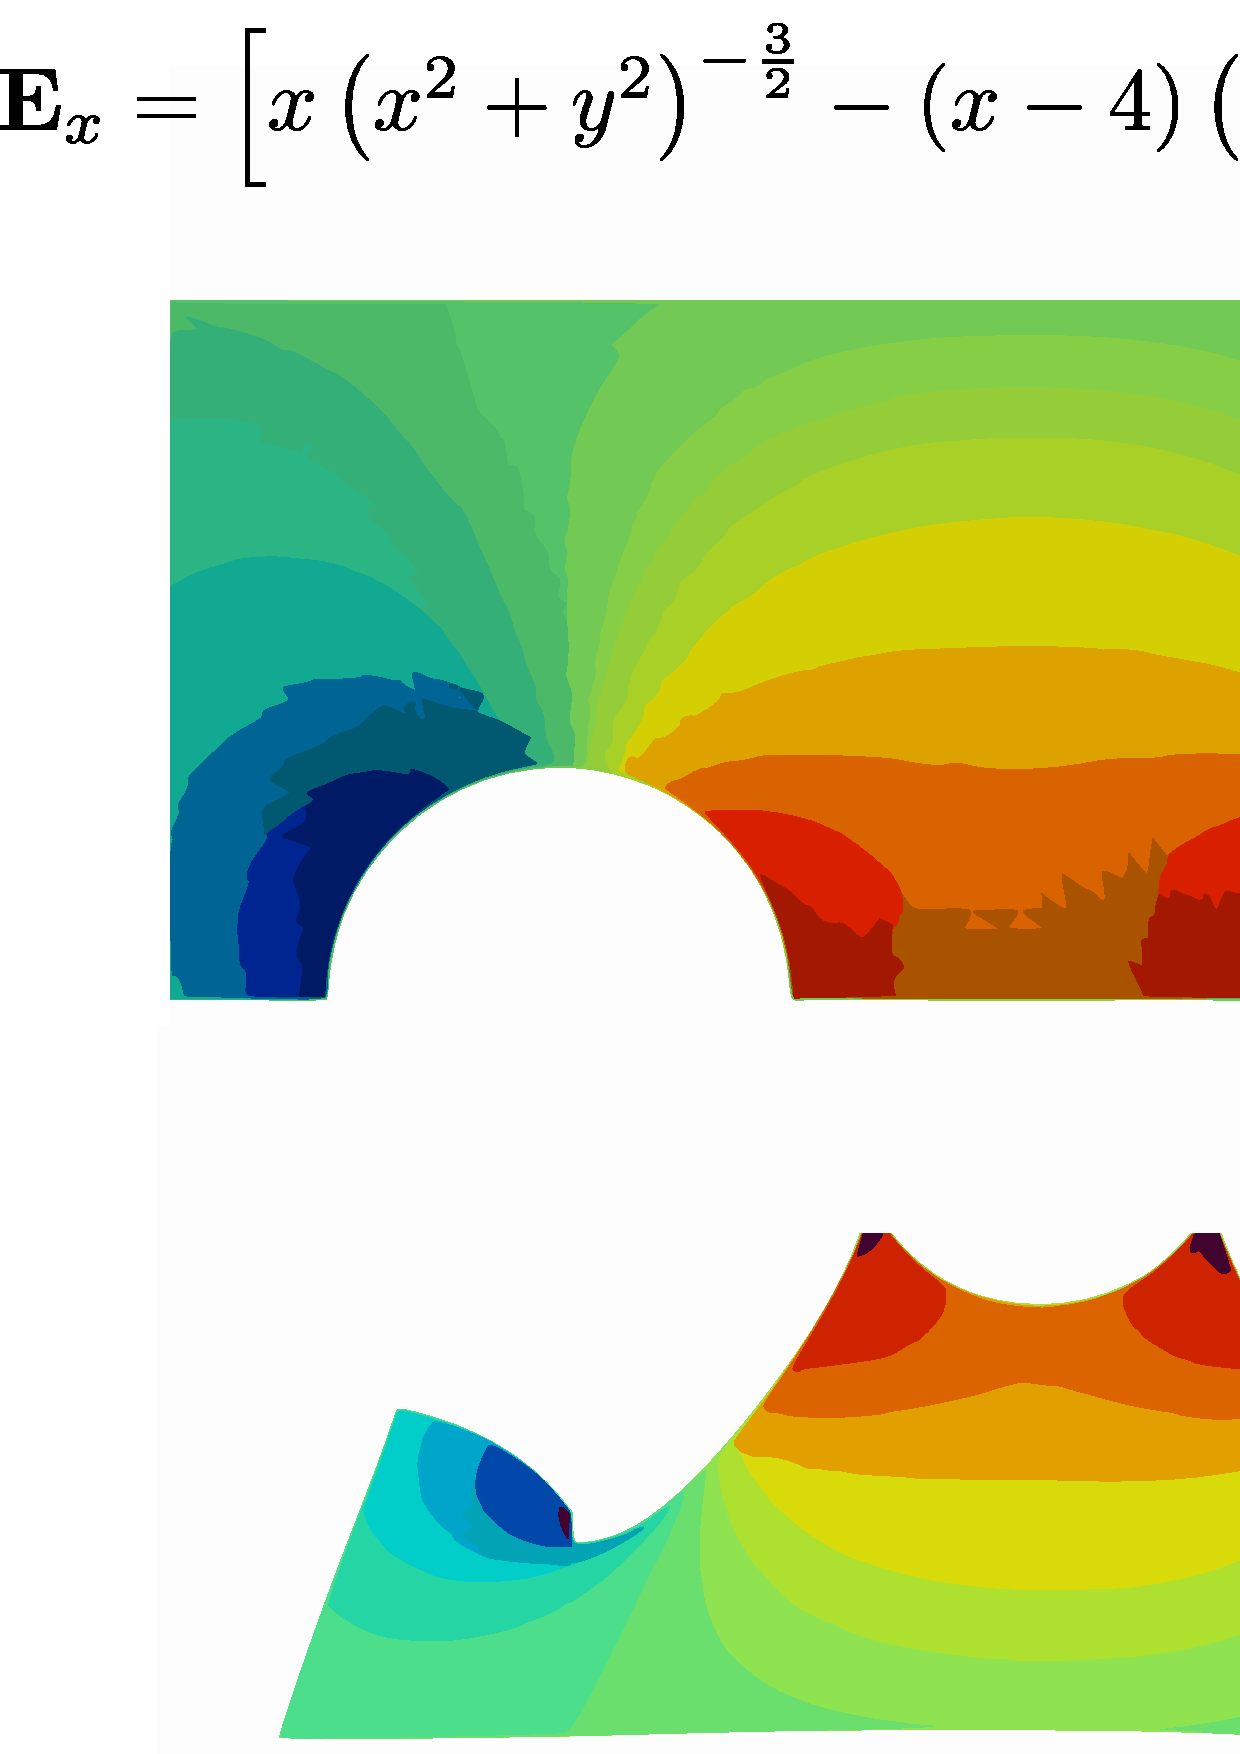
\includegraphics[scale=0.2]{./img/two_cylinders.pdf}
\caption{Components of the electric field after simulating a problem of two cylinders with opposite charges.}
\label{fig:two_cylinders}
\end{figure}

\begin{figure}
\centering
\includegraphics[scale=0.5]{./img/two_cylinders_Gliphs}
\caption{Arrow glyphs of the solution for the dipole problem. Lenght and color of the arrow indicate magnitude of the field. As expected, the field points from the positively charged cylinder to the negative.}
\label{fig:two_cylinders_glyph}
\end{figure}

\begin{figure}
\centering
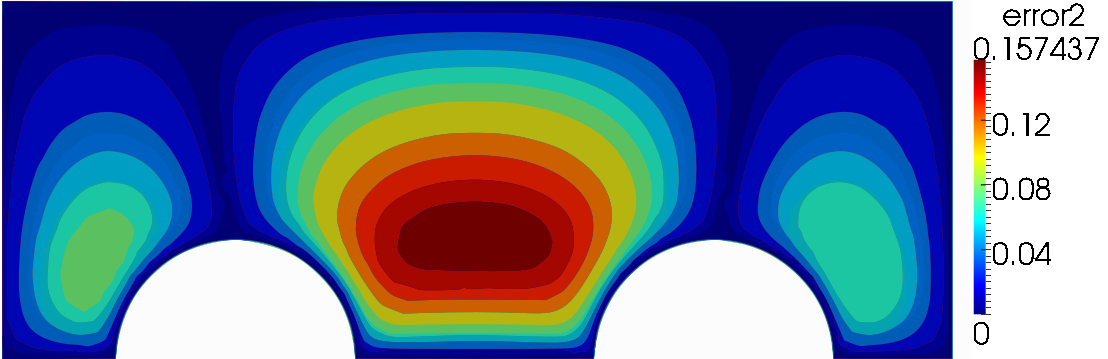
\includegraphics[scale=0.4]{./img/two_cylinders_error.pdf}
\caption{Error calculation of simulation against exact solution. The method reproduces the nature of the problem, but a finer mesh is needed to obtain precise results.}
\label{fig:two_cylinders_error}
\end{figure}

\section{Harmonic benchmark tests}
The second section regards solutions of eigenvalue problems, either for closed domains or infinite and periodic ones. The first part will deal with simulation of resonant modes in wave guides, and the second with free waves and periodic crystals.

\subsection{Eigenvalues and modes in waveguides}

Ideal wave guides can be modelled by a source-less version of the wave equation for time harmonic fields \ref{eq:E-wave-harmonic} in arbitrary 2D domains closed by a metallic boundary that guarantees Dirichlet condition $\mathbf{E} = 0\quad at\quad \Gamma$. This problem is relevant in electromagnetism and telecommunications because it is the principle behind many applications such as data transmission in fiber optics, and microwaves. Here, the 2D domain represents a cross section of a metallic structure that guides waves along its axis. We are particularly interested in knowing two things:
\begin{enumerate}
\item The modes or wave functions that are solution to the equation for a particular shape.
\item The frequencies associated to those modes or shapes. 
\end{enumerate}
And will start by introducing the analytic solution behind simple wave guides such as rectangular and circular guides.

\subsubsection{Rectangular waveguides} 

In transverse magnetic fields (TM) that travel inside a waveguide whose axis is over $z$, we have $\mathbf{H}_z = 0$ and solve for $\mathbf{E}$ components. 
Solutions of equation \ref{eq:E-wave-harmonic2} where the medium inside the wave guide is a perfect dielectric, and  for eigenvalues $\vec{k}^2 = \omega^2\mu\epsilon$ is a lengthy but straightforward process that involves separation of variables and use of boundary conditions:
\begin{align}
&\mathbf{E}_x = 0 \quad for \quad y=0,\ 0<x<a\\
&\mathbf{E}_x = 0 \quad for \quad y=b,\ 0<x<a\\
&\mathbf{E}_y = 0 \quad for \quad x=0,\ 0<y<b\\
&\mathbf{E}_y = 0 \quad for \quad x=a,\ 0<y<b
\end{align}

A description of the solution process is left for the reader to look up in references such as Rao  \cite{Rao2004} or Jianming \cite{Jin2010}. What is found in the process is that only certain discrete frequencies are allowed inside the waveguide, and they are given by:

\begin{equation}
\omega_{n,m} = \frac{1}{\sqrt{\mu\epsilon}}\sqrt{\left(\frac{m\pi}{a}\right)^2+\left(\frac{n\pi}{b}\right)^2}
\qquad m,n = 0,1,2,... \quad (m=n\neq0)
\label{eq:eig_vals_sqare_waveguide}
\end{equation}
Where $\omega$ is indexed by integers $n,m$ and the trivial solution $\omega = 0$ is excluded. $a$ is the width of the rectangular cross section and $b$ is its height.
The wave functions that are solution to this eigenproblem for each component of the field are in the following general form:

\begin{align}
&\mathbf{E}_z = A\sin{\dfrac{m\pi x}{a}}\sin{\dfrac{n\pi x}{b}}e^{\mp jk_zz} \label{eq:Ez_mag}\\
&\mathbf{E}_x =\mp jB\dfrac{m\pi}{a}\cos{\dfrac{m\pi x}{a}}\sin{\dfrac{n\pi x}{b}}e^{\mp jk_zz}\\
&\mathbf{E}_y =\mp jC\dfrac{n\pi}{b}\sin{\dfrac{m\pi x}{a}}\cos{\dfrac{n\pi x}{b}}e^{\mp jk_zz}
\end{align}

For our comparisons we will only look at how closely the shapes of the simulated solution represent $\mathbf{E}$ in \ref{eq:Ez_mag}, and how similar are the analytic and numeric  natural frequencies of the guide $\omega$.


\begin{figure}
\centering

\includegraphics[scale=0.1]{./img/square_waveguide.pdf}
\caption{Results for three different modes from the simulation of a square shaped waveguide with side $a=b=2$}
\label{fig:square_waveguide}
\end{figure}

\chapter{Conclusions and future work}

\section{Conclusions}
The objectives were met.

\section{Future work}
\begin{itemize}
\item Define vectorial triangular elements and scalar quadrilateral elements.
\item Consider adding regions with Perfectly Matched Layers (PML) for the simulation of
	  open domains.
\item Evaluate convergence of the method for the problems described in chapter \ref{ch:Results} using finer spatial and spectral meshes. 
\item Perform more simulations of time dependent problems involving deffects in finite crystals. And compare the results of Q factor and efficiency with other publications.
\item Integrate the CAD and solver into a optimization algorithm that maximizes transmission or confinement by inducing variations in position and shape of defects in the lattice.
\item Consider parallelization schemes to be implemented in order to make bigger simulations plausible.
\end{itemize}




\cleardoublepage \phantomsection
\addcontentsline{toc}{chapter}{References}
\bibliographystyle{unsrt}
\bibliography{thesis_references}
\end{document}